% ============================================================================
% Beyond Pareto Fronts: A Leximax Universal-Regret Core for Robust
% Multicriteria Decision Support
%
% Formatted in the standard article class for portable compilation.
% For final EJOR submission, switch the first line to
%   \documentclass[review]{elsarticle}
% and move the abstract/keywords into the elsarticle frontmatter; the body,
% theorems, tables and figures below transfer unchanged.
% ============================================================================
\documentclass[review]{elsarticle}

\usepackage[a4paper,margin=1in]{geometry}
\usepackage{amsmath,amssymb,amsthm,mathtools}
\usepackage{graphicx}
\usepackage{booktabs}
\usepackage{xcolor}
\usepackage{caption}
\usepackage{subcaption}
\usepackage{pifont}
\usepackage{tikz}
\usetikzlibrary{arrows.meta,positioning,fit,backgrounds,shapes.geometric,shapes.arrows,calc,matrix}
\usepackage[hidelinks]{hyperref}
\usepackage{setspace}
\onehalfspacing

\graphicspath{{./}{./figures/}}

% ---- shared TikZ styles for the schematic figures ----
\definecolor{lurcrimson}{HTML}{C0392B}
\definecolor{lurslate}{HTML}{34495E}
\definecolor{lurblue}{HTML}{2980B9}
\definecolor{lurgreen}{HTML}{27AE60}
\tikzset{
  stage/.style={rounded corners=2pt, draw=lurslate, line width=0.6pt,
    fill=lurslate!6, align=center, inner sep=5pt, font=\small},
  accent/.style={rounded corners=2pt, draw=lurblue, line width=0.7pt,
    fill=lurblue!8, align=center, inner sep=5pt, font=\small},
  win/.style={rounded corners=2pt, draw=lurcrimson, line width=0.9pt,
    fill=lurcrimson!8, align=center, inner sep=5pt, font=\small},
  flow/.style={-{Stealth[length=2.4mm]}, line width=0.7pt, draw=lurslate},
}

\newtheorem{theorem}{Theorem}
\newtheorem{corollary}{Corollary}
\newtheorem{lemma}{Lemma}
\newtheorem{definition}{Definition}
\newtheorem{proposition}{Proposition}
\theoremstyle{remark}
\newtheorem{remark}{Remark}

\newcommand{\R}{\mathbb{R}}
\newcommand{\Q}{\mathcal{Q}}
\newcommand{\X}{\mathcal{X}}
\newcommand{\reg}{D}
\newcommand{\ideal}{z^{\star}}
\newcommand{\nadir}{z^{nad}}
\newcommand{\lex}{\leq_{\mathrm{lex}}}
\DeclareMathOperator*{\argmin}{arg\,min}
\DeclareMathOperator*{\argmax}{arg\,max}
\DeclareMathOperator{\Corr}{Corr}

\IfFileExists{generated/protocol_numbers.tex}{\input{generated/protocol_numbers.tex}}{
  \newcommand{\protocolInstances}{7,200}
  \newcommand{\protocolMethods}{11}
  \newcommand{\protocolCD}{0.31}
}

\begin{document}
\begin{frontmatter}
\title{\textbf{Beyond Pareto Fronts: A Leximax Universal-Regret Core\\
for Robust Multicriteria Decision Support}}
\author{Madani Bezoui}
\address{CESI LINEACT, UR 7527}
\begin{abstract}
\noindent
Pareto efficiency is necessary but not sufficient for a unique recommendation. An
efficient set tells a decision maker (DM) which alternatives are not obviously
bad, but offers no principled way to choose one. Practice fills this gap with
\emph{post hoc} devices---weighted sums, TOPSIS, compromise programming,
reference points, acceptability indices---each injecting implicit or stochastic
preference judgements.

We propose the \textbf{Leximax Universal-Regret (LUR) core}, a leximin-refined preference-robust selection rule operating over a structured, declared, monotone scalarisation family. The
DM defines an explicit family of rational questions (probes) and supplies normalisation bounds. 
LUR treats each probe's evaluation as an achievement function, calculating how far each alternative
falls from the best attainable outcome under each probe, and sorts the resulting
dimensionless regrets. The alternative whose worst performance is best is
recommended, with an interpretable certificate listing the binding questions. 

We prove existence and completeness, Pareto compatibility, stability of the
tolerance-based leximax rule under bounded perturbations, and a probe
perturbation bound with explicit constants. We also give an adaptive
correlation-clustering construction empirically reducing, without eliminating,
sensitivity to redundant criteria.

In a replicated benchmark and a frozen audit
broadened protocol covering 11 methods, 10 held-out preference families, 8 front
geometries, and $m$ up to 20, LUR sits in the best-performing group on tail held-out loss. Its distinct empirical advantages over averaging methods are its interpretable certificate and reduced redundancy bias. Because the exact identity of the lexicographic minimiser can be highly sensitive to estimated normalisation bounds, the framework's primary robust deliverable is a \emph{stability set} (or indifference class) evaluated over conservative interval bounds, with a unique point recommendation returning as a special case when verified margin conditions hold. We formulate an exploratory stochastic extension illustrated on a synthetic smart-grid economic dispatch model.
\end{abstract}

\begin{keyword}
Decision support \sep Multicriteria decision analysis \sep
Robust decision making \sep Minimax regret \sep Achievement scalarising functions \sep
Pareto efficiency
\end{keyword}
\end{frontmatter}

% ---------------------------------------------------------------------------
\section{Introduction}
\label{sec:intro}

Since the work of Pareto, efficiency has been the cornerstone of multicriteria analysis: an alternative is Pareto efficient if no criterion can be improved without worsening another. This is a safety property that removes dominated alternatives, but it is decisionally incomplete. For $m$ conflicting criteria the efficient set is typically large, leaving the decision maker (DM) with no principled selection rule. The fundamental issue remains that the Pareto front is a safety filter, not a complete decision rule.

LexUR turns the output from a set into a certified recommendation. The DM declares a monotone probe family and normalization bounds. Each alternative receives normalized regrets over that family. These regrets are lexicographically sorted, and selection follows a lexicographic minimax rule. This yields a certified stability class accompanied by an explanation of which questions remain most severely binding. Figure~\ref{fig:paretocert} contrasts the safety filter with the regret certificate.

% From a Pareto front (safety filter) to a regret certificate (decision)
\begin{figure}[t]
\centering
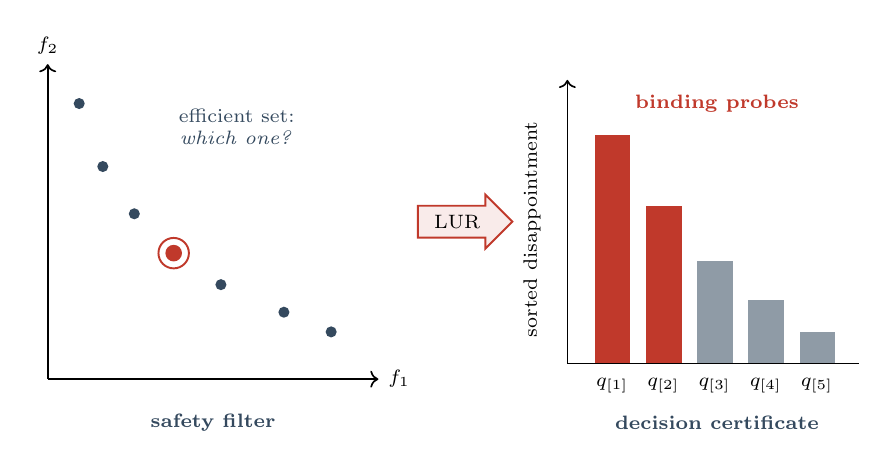
\begin{tikzpicture}
% ---------- left panel: efficient front ----------
\begin{scope}
\draw[->, line width=0.6pt] (0,0) -- (4.2,0) node[right, font=\scriptsize] {$f_1$};
\draw[->, line width=0.6pt] (0,0) -- (0,4.0) node[above, font=\scriptsize] {$f_2$};
% convex-ish front of points
\foreach \x/\y in {0.4/3.5, 0.7/2.7, 1.1/2.1, 1.6/1.6, 2.2/1.2, 3.0/0.85, 3.6/0.6}{
  \fill[lurslate] (\x,\y) circle (2.0pt);
}
\node[lurslate, font=\scriptsize, align=center] at (2.4,3.2) {efficient set:\\\emph{which one?}};
\node[font=\scriptsize\bfseries, lurslate] at (2.1,-0.55) {safety filter};
% highlight chosen point
\fill[lurcrimson] (1.6,1.6) circle (3.0pt);
\draw[lurcrimson, line width=0.7pt] (1.6,1.6) circle (5.5pt);
\end{scope}

% ---------- arrow ----------
\node[flow, single arrow, draw=lurcrimson, fill=lurcrimson!10, minimum height=12mm,
      single arrow head extend=1.4mm, inner sep=3pt, font=\scriptsize, align=center]
      at (5.2,2.0) {LUR};

% ---------- right panel: certificate ----------
\begin{scope}[xshift=6.6cm, yshift=0.2cm]
\draw[->, line width=0.6pt] (0,0) -- (0,3.6) node[above, font=\scriptsize] {};
\node[font=\scriptsize, rotate=90] at (-0.45,1.7) {sorted disappointment};
\foreach \i/\h/\lab in {0/2.9/$q_{[1]}$, 1/2.0/$q_{[2]}$, 2/1.3/$q_{[3]}$, 3/0.8/$q_{[4]}$, 4/0.4/$q_{[5]}$}{
  \pgfmathsetmacro\xx{0.35+\i*0.65}
  \ifnum\i<2
    \fill[lurcrimson] (\xx,0) rectangle ++(0.45,\h);
  \else
    \fill[lurslate!55] (\xx,0) rectangle ++(0.45,\h);
  \fi
  \node[font=\scriptsize] at (\xx+0.22,-0.28) {\lab};
}
\draw[line width=0.6pt] (0,0) -- (3.7,0);
\node[lurcrimson, font=\scriptsize\bfseries, align=center] at (1.9,3.3) {binding probes};
\node[font=\scriptsize\bfseries, lurslate] at (1.9,-0.75) {decision certificate};
\end{scope}
\end{tikzpicture}
\caption{From a front to a certificate. The efficient set (left) removes dominated
options but leaves the choice open. LUR returns one alternative together with its
sorted regret certificate (right), whose largest entries---the \emph{binding
probes}---explain where the recommendation remains most fragile.}
\label{fig:paretocert}
\end{figure}


Our contributions are unified across four dimensions. Theoretically, we define the LexUR order and prove existence, completeness, Pareto compatibility, and stability under bounded perturbations. Algorithmically, we provide an exact finite-set procedure using sequential sorts. Empirically, we validate LexUR on a broadened benchmark suite, demonstrating competitive tail performance against strong robust baselines. Interpretably, we introduce an adaptive correlation-clustering probe family that handles redundancy and produces an auditable regret certificate for the final choice.

Robustness in this framework is strictly relative to the declared probe family, not all possible preferences. Furthermore, point normalization may be sensitive when ideal and nadir bounds are uncertain. LexUR is not parameter-free, but its assumptions are declared, auditable, and separated from the final recommendation.

Section~\ref{sec:related} positions the method. Sections~\ref{sec:core} to~\ref{sec:probes} develop the core theory, computation, and probe design. Sections~\ref{sec:ext} and~\ref{sec:exp} test extensions and empirical performance, and Section~\ref{sec:disc} closes with implications.

\section{Background and related work}
\label{sec:related}

\subsection{Pareto efficiency and \emph{post hoc} selection}
For a vector objective $F(x)=(f_1(x),\dots,f_m(x))$ (minimisation), $x$
Pareto-dominates $y$ if $f_i(x)\le f_i(y)$ for all $i$ with at least one strict
inequality; the efficient set is the non-dominated set. Because it is typically
large, a single recommendation is obtained by \emph{post hoc} selection. The
weighted sum, TOPSIS \citep{hwang1981}, compromise programming
\citep{zeleny1982}, knee selection \citep{branke2008}, ELECTRE \citep{roy1968,roy1991},
PROMETHEE \citep{brans2016} and hypervolume selection \citep{zitzler1999} are the
standard tools; each requires weights, thresholds, a metric, or an already
generated front. LexUR does not eliminate modelling choices. It relocates them into a declared family of admissible monotone probes and, on finite candidate sets, computes the resulting recommendation exactly while returning a labelled regret certificate.

\subsection{Achievement scalarising functions and ordered aggregation}
Achievement scalarising functions (ASF) project a reference point onto the
efficient set through a parameterised metric interpolating between $L_1$ and
$L_\infty$ \citep{wierzbicki1980,miettinen2002}. Ordered weighted averaging
(OWA) \citep{yager1988} and its extensions (WOWA) \citep{torra1997}
connect ordered aggregation to lexicographic maximin. 

\begin{remark}[Recovery of standard scalarisations]
\label{rem:special}
The LexUR core recovers standard aggregation methods as exact special cases under specific, restricted probe families:
\begin{itemize}
\item \textbf{Weighted sum:} If $\Q=\{q_w(r)=w^\top r\}$, LexUR exactly minimises the weighted sum of normalised criteria.
\item \textbf{Chebyshev / ASF:} If $\Q=\{q_w(r)=\max_i w_i r_i\}$, LexUR exactly minimises the Chebyshev distance to the ideal point.
\item \textbf{Lexicographic minimax:} If $\Q=\{r_1,\dots,r_m\}$ (the singleton family), LexUR performs a lexicographic minimax optimisation over the normalised regrets.
\end{itemize}
\end{remark}

We do not claim
LexUR subsumes these methods with its full adaptive family---there it is a
\emph{different} aggregation paradigm. Its distinguishing features are that it
sorts \emph{normalised regrets} (dimensionless disappointments relative to each
probe's own attainable best and worst) over a \emph{declared family of probes}
and breaks ties through the whole sorted vector, and that it emits a certificate.

\subsection{Robust MCDA: SMAA, robust ordinal regression, preference robust
optimisation}
The work closest to LexUR lies in \emph{robust} multicriteria decision analysis and minimax regret optimisation \citep{kouvelis1997}.
\textbf{SMAA} \citep{lahdelma1998,tervonen2007} computes, by Monte-Carlo
integration over a distribution of admissible weights (and possibly criterion
values), acceptability indices describing how strongly each alternative is
supported. \textbf{Robust ordinal regression} \citep{greco2008,figueira2009}
reasons over the entire set of additive value functions compatible with a DM's
holistic pairwise judgements, producing necessary and possible preference
relations, sharing goals with inverse MCDA and the UTA family \citep{jacquetlagreze1982}. \textbf{Preference robust optimisation} \citep{armbruster2015,hu2015,delage2015,vayanos2020}
optimises the worst-case expected utility over an ambiguity set of utility
functions. LexUR shares the robust philosophy---perform well across a whole class of
admissible preferences rather than commit to one---but differs in three ways.
First, its admissible class is an explicit family of \emph{monotone probes}, not a
weight distribution or an elicited polyhedron. Second, its criterion is the
\emph{lexicographic minimax of normalised regret}, not an expected acceptability,
a necessary/possible relation, or a single worst-case utility. Third, its output
is an interpretable \emph{certificate} naming the binding coalitions. We note that
SMAA is inherently an \emph{exploratory} framework designed to visualise the robustness of alternatives across weight spaces, rather than a single-choice prescriptive rule. By forcing it to recommend the alternative with the highest first-rank acceptability index (ties broken by expected value), we create a comparable baseline for \S\ref{sec:exp}; however, we emphasise that LexUR's single-shot default recommendation is meant to \emph{complement} rather than compete with SMAA's rich exploratory indices. We likewise compare against a Savage minimax-regret (MMR)
recommender over a sampled linear weight set (\S\ref{sec:exp}). More broadly, LexUR
is complementary to data-driven preference disaggregation and inverse MCDA
\citep{doumpos2011}, which infer preference parameters from holistic judgements:
LexUR instead dispenses with a fitted preference model and reasons over a declared
class of questions, and could take an elicited probe family as input where such
data exist.

\subsection{Minimax regret and robust optimisation}
Regret-based choice originates with \citet{savage1951} and \citet{loomes1982};
minimax regret seeks alternatives minimising the largest shortfall from the best
attainable value. Robust optimisation \citep{bental2002} and stochastic
programming \citep{birge2011} address parameter uncertainty in the model rather
than preference uncertainty in the DM. LexUR extends minimax regret in three
directions: it is \emph{lexicographic} (after the worst regret, minimise the
second worst, and so on), \emph{probe-based} (regret is computed over rational
coalitions of criteria, not raw criteria), and \emph{direct on a given candidate
set} (computed without an additional scalarisation sweep, and front-free only in
the structured continuous cases of \S\ref{sec:direct}).

\subsection{Social choice and fairness}
Aggregating criteria resembles social choice, but treating criteria as voters
invites Condorcet cycles; LexUR avoids this by aggregating \emph{regrets over
declared questions}, not votes over criteria. For multi-stakeholder settings we
draw on the maximin principle of \citet{rawls1971} and the bargaining viewpoint
of \citet{nash1950}; we claim natural fairness properties (anonymity, monotonicity,
worst-stakeholder protection), not a uniqueness theorem.

\subsection{What is new relative to existing regret and robust-MCDA rules}
\label{sec:novelty}

While LexUR shares motivation with several robust approaches, its mathematical object and output differ fundamentally:
\begin{itemize}
\item \textbf{Versus minimax regret:} LexUR minimises a sorted vector of normalised probe regrets, not a single maximum regret over raw utilities or sampled weights.
\item \textbf{Versus ASF/Chebyshev:} ASF commits to one scalarising function or one reference structure; LexUR evaluates a declared family and certifies binding probes.
\item \textbf{Versus SMAA:} SMAA integrates over a preference distribution and reports acceptability; LexUR does not require a probability distribution and returns a leximax regret certificate.
\item \textbf{Versus robust ordinal regression (ROR):} ROR reasons over compatible value functions after elicited comparisons; LexUR can operate without holistic preference judgements.
\item \textbf{Versus preference robust optimisation (PRO):} PRO optimises worst-case utility over an ambiguity set; LexUR optimises lexicographically sorted normalised disappointments over interpretable monotone probes.
\item \textbf{Versus ordered weighted aggregation (OWA):} LexUR sorts regrets
across declared questions, not criterion values themselves. OWA specifies an
ordered weight vector, whereas LexUR specifies a probe family; both therefore
encode modelling choices in different forms. We include OWA utilities as a
held-out evaluation family, not as evidence that LexUR subsumes OWA.
\end{itemize}

The novelty is not minimax regret alone, but lexicographic minimax over normalised disappointments induced by a declared monotone probe family, with an auditable certificate and an adaptive redundancy-aware probe construction.

Table~\ref{tab:positioning} summarises where LexUR sits relative to representative MCDA and robust methods.

\begin{table}[t]
\centering\small
\caption{Comparison of LexUR with representative selection and robust-MCDA methods.}
\label{tab:positioning}
\begin{tabular}{p{2.2cm}p{3.2cm}p{1.3cm}p{2.6cm}p{3.7cm}}
\toprule
Method & Required Input & Pareto Comp. & Output / Explanation & Key Limitation \\
\midrule
Weighted sum & Weight vector & Yes ($w>0$) & Single choice (Low) & Misses non-supported points in non-convex fronts \\
TOPSIS & Weights, distance metric & Not strictly & Single choice (Low) & Rank reversal; distance to non-feasible ideal \\
CP & Weights, $L_p$ exponent & Yes ($p<\infty$) & Single choice (Low) & Non-linear scaling effects \\
ASF / Chebyshev & Reference point, scaling & Yes & Single choice (Low) & Requires an arbitrary reference point \\
MMR (sampled) & Linear weight distribution & Yes & Worst-case regret & Limited to linear aggregations \\
SMAA & Preference distribution & Usually & Acceptability indices & Exploratory; single-choice depends on post-processing \\
VIKOR & Weights, majority threshold & Not strictly & Single choice (Low) & Complex parameter interaction \\
Single-point HV & Reference point & Yes & Single choice (Low) & Box-volume score; sensitive to reference point \\
\textbf{LexUR (ours)} & Monotone probe family & Yes\textsuperscript{*} & Leximax certificate & Sensitive to normalisation bounds \\
\bottomrule
\multicolumn{5}{l}{\footnotesize \textsuperscript{*} Strict Pareto compatibility holds if probes separate criteria (Theorem~\ref{thm:pareto}).}
\end{tabular}
\end{table}

\section{The Leximax Universal-Regret core}
\label{sec:core}

Figure~\ref{fig:pipeline} gives the end-to-end view of the rule developed in this
section: from a candidate set, through normalisation and the declared probe family,
to the leximax selection and its certificate.

% LUR end-to-end pipeline schematic
\begin{figure}[t]
\centering
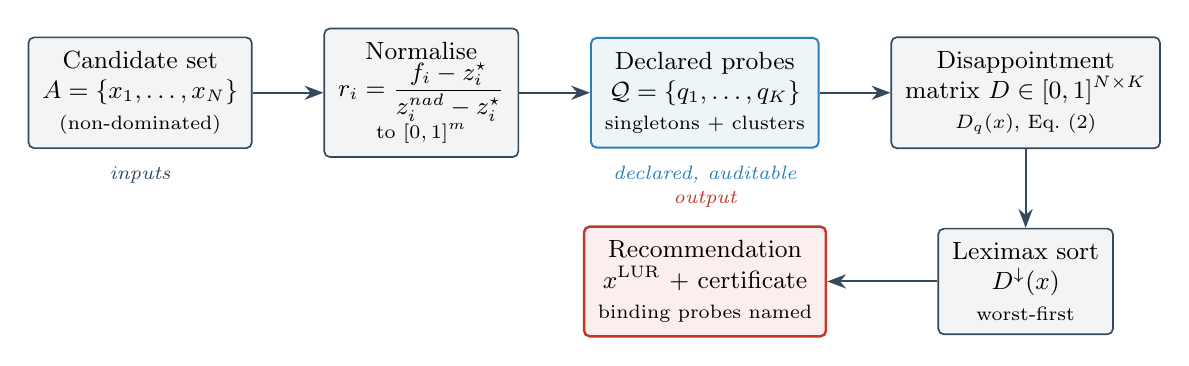
\begin{tikzpicture}[node distance=6mm and 9mm]
\node[stage] (A) {Candidate set\\$A=\{x_1,\dots,x_N\}$\\\scriptsize(non-dominated)};
\node[stage, right=of A] (N) {Normalise\\$r_i=\dfrac{f_i-\ideal_i}{\nadir_i-\ideal_i}$\\\scriptsize to $[0,1]^m$};
\node[accent, right=of N] (Q) {Declared probes\\$\Q=\{q_1,\dots,q_K\}$\\\scriptsize singletons + clusters};
\node[stage, right=of Q] (D) {Disappointment\\matrix $\reg\in[0,1]^{N\times K}$\\\scriptsize $\reg_q(x)$, Eq.~(2)};
\node[stage, below=10mm of D] (S) {Leximax sort\\$\reg^{\downarrow}(x)$\\\scriptsize worst-first};
\node[win, left=14mm of S] (W) {Recommendation\\$x^{\mathrm{LUR}}$ + certificate\\\scriptsize binding probes named};

\draw[flow] (A) -- (N);
\draw[flow] (N) -- (Q);
\draw[flow] (Q) -- (D);
\draw[flow] (D) -- (S);
\draw[flow] (S) -- (W);

\node[font=\scriptsize\itshape, lurslate, below=1mm of A] {inputs};
\node[font=\scriptsize\itshape, lurblue, below=1mm of Q] {declared, auditable};
\node[font=\scriptsize\itshape, lurcrimson, above=1mm of W] {output};
\end{tikzpicture}
\caption{The LUR pipeline. Modelling choices are confined to the \emph{declared}
probe family $\Q$ and the normalisation bounds; the selection itself is an exact,
deterministic leximax over the disappointment matrix, and the output is a single
recommendation accompanied by an auditable regret certificate.}
\label{fig:pipeline}
\end{figure}


\subsection{Problem setting and normalisation}
Let $\X\subseteq\R^n$ be the feasible set and $F:\X\to\R^m$, $F(x)=(f_1(x),\dots,
f_m(x))$, the vector objective.

\begin{center}
\fbox{
\begin{minipage}{0.9\columnwidth}
\textbf{Convention:} All criteria $f_i$ are assumed to be \emph{minimised}. Maximisation objectives must have their sign reversed before normalisation. Consequently, lower normalised values $r_i$ are better, and probes are non-decreasing functions of these costs.
\end{minipage}
}
\end{center}

For
the finite case let $A=\{x_1,\dots,x_N\}\subseteq\X$ be a candidate set, e.g.\ an
\emph{a posteriori} approximation of the efficient set. Before evaluation, Pareto-dominated alternatives are removed from $A$ unless the analyst explicitly requires selection over the raw un-filtered set. For the continuous case (\S\ref{sec:direct}) $A$ is not required. Criteria are normalised to $[0,1]$ by the
positive affine map
\begin{equation}
r_i(x)=\frac{f_i(x)-\ideal_i}{\nadir_i-\ideal_i},\qquad
\ideal_i=\min_{x\in A}f_i(x),\;\; \nadir_i=\max_{x\in A}f_i(x),
\label{eq:norm}
\end{equation}
which attains both endpoints on $A$. A criterion is flagged as numerically degenerate if the range $\nadir_i-\ideal_i$ approaches zero. Degenerate criteria are reported and excluded from non-singleton probe construction unless the analyst supplies external bounds.

For the finite case all extrema ($\ideal$,
$\nadir$, $q^\star$, $q^{\mathrm w}$ below) are taken over the active candidate set $A$;
for the continuous case (\S\ref{sec:direct}) they are taken over $\X$. We use the
upper attainable value over $A$ in place of the true nadir over the efficient
set; the two coincide when $A$ contains the criterion-wise worst efficient points,
and otherwise the former is a conservative upper normalisation bound. The rule is invariant to
positive affine rescaling of the criteria when the bounds are transformed
consistently; it is not invariant to arbitrary monotone transformations (e.g.\
$f_i\mapsto\log f_i$), which change the distances that define regret---so such
transformations are a modelling choice the analyst must make deliberately.

\subsection{Admissible probes}
A \emph{probe} is a scalar function $q:[0,1]^m\to\R$ encoding a rational decision
question. The family $\Q$ is \emph{declared}: it is part of the specification.

\begin{definition}[Admissible probe]
\label{def:probe}
A probe $q$ is \emph{admissible} if (i) it is non-decreasing in each $r_i$
(monotonicity) and (ii) it can be rescaled so that $q(\mathbf 0)=0$, $q(\mathbf
1)=1$ (normalisation).
\end{definition}

Here $\mathbf 0$ and $\mathbf 1$ denote the all-zeros and all-ones vectors. The initial endpoint normalisation ($q(\mathbf 0)=0, q(\mathbf 1)=1$) serves to make values structurally scale-comparable across the heterogeneous family, before the empirical disappointment anchors ($q^\star, q^{\mathrm w}$) re-normalise the observed active range.
Monotonicity gives \emph{weak} Pareto compatibility; strict compatibility needs a
separation property (Definition~\ref{def:sep}). Canonical admissible probes are
the \emph{singletons} $q_i(r)=r_i$; the \emph{grand mean} $q_\mu(r)=\frac1m
\sum_i r_i$ (the utilitarian question); the \emph{grand maximum}
$q_{\max}(r)=\max_i r_i$ (the egalitarian/worst-criterion question); and, for any
coalition $S\subseteq\{1,\dots,m\}$, the coalition mean and maximum. All have
non-negative weights or are maxima, hence are monotone.

\begin{definition}[Separating family]
\label{def:sep}
A probe family $\Q$ \emph{separates} criteria if for every $i$ there is a probe
$q\in\Q$ strictly increasing in $r_i$. Including all $m$ singleton probes
$q_i(r)=r_i$ is sufficient; LUR always does so.
\end{definition}

\subsection{Disappointment and regret}
For each probe $q\in\Q$ let $q^\star=\min_{x\in A}q(r(x))$ and $q^{\mathrm w}=\max_{x\in A}q(r(x))$
(or a user-supplied worst-acceptable bound). Define the active range $R_q = q^{\mathrm w} - q^\star$. If $R_q < \varepsilon_q$ for a small numerical threshold, the probe is degenerate and is excluded from the primary decision vector. Otherwise, the \emph{normalised disappointment} of $x$ under $q$ is
\begin{equation}
\reg_q(x)=\frac{q(r(x))-q^\star}{R_q}\in[0,1],
\label{eq:disap}
\end{equation}
so that $\reg_q(x)=0$ iff $x$ is $q$-optimal and $1$ iff $x$ attains the worst bound.

We use the term \emph{disappointment} for the normalised shortfall of an alternative from the best attainable value of a single given probe, and \emph{regret certificate} for the vector collecting these probe-wise disappointments. This is regret-like but differs from classical pairwise Savage regret unless the probe family is interpreted specifically as the uncertainty set of possible true preference functions.

\subsection{The leximax order}
Collect $\reg(x)=(\reg_{q_1}(x),\dots,\reg_{q_K}(x))$, $K=|\Q|$, and sort it in
\emph{descending} order to obtain $\reg^{\downarrow}(x)=(\reg_{[1]}(x)\ge\dots\ge
\reg_{[K]}(x))$. The \textbf{Leximax Universal-Regret order} is
\begin{equation}
x\preceq_{\mathrm{LUR}}y \iff \reg^{\downarrow}(x)\lex \reg^{\downarrow}(y),
\label{eq:lur}
\end{equation}
i.e.\ $x$ is preferred if its worst disappointment is smaller; on ties, its
second worst; and so on. The \emph{LUR solution} is $x^{\mathrm{LUR}}\in
\argmin^{\mathrm{lex}}_{x}\reg^{\downarrow}(x)$, and its \emph{certificate} is the
labelled, sorted vector $\reg^{\downarrow}(x^{\mathrm{LUR}})$ together with the
probes attaining the largest entries. Figure~\ref{fig:leximax} illustrates the
comparison on a two-alternative example.

% Leximax comparison of two alternatives' sorted disappointment vectors
\begin{figure}[t]
\centering
\begin{tikzpicture}[x=1cm, y=1cm]
\def\barw{0.42}
\def\sc{0.8}        % vertical scale for bar heights
\def\rowA{3.0}      % baseline y for row A
\def\rowB{1.6}      % baseline y for row B
\def\Lx{0}          % left block origin x
\def\Rx{4.8}        % right block origin x

% --- column titles ---
\node[font=\scriptsize\bfseries] at (\Lx+1.1,4.45) {unsorted regrets};
\node[font=\scriptsize\bfseries] at (\Rx+1.1,4.45) {sorted $\reg^{\downarrow}$ (worst-first)};

% --- row labels ---
\node[font=\small, anchor=east] at (\Lx-0.15,\rowA+0.3) {$A$};
\node[font=\small, anchor=east] at (\Lx-0.15,\rowB+0.3) {$B$};
\node[font=\small, anchor=east] at (\Rx-0.15,\rowA+0.3) {$A$};
\node[font=\small, anchor=east] at (\Rx-0.15,\rowB+0.3) {$B$};

% --- unsorted bars ---
\foreach \v/\i in {0.2/0,0.9/1,0.4/2,0.7/3,0.3/4}{
  \fill[lexurslate!50] (\Lx+\i*0.5,\rowA) rectangle ++(\barw,{\v*\sc});}
\foreach \v/\i in {0.6/0,0.8/1,0.5/2,0.8/3,0.2/4}{
  \fill[lexurslate!50] (\Lx+\i*0.5,\rowB) rectangle ++(\barw,{\v*\sc});}

% --- sorted bars (A wins/loses comparison) ---
\foreach \v/\i in {0.9/0,0.7/1,0.4/2,0.3/3,0.2/4}{
  \fill[lexurslate!50] (\Rx+\i*0.5,\rowA) rectangle ++(\barw,{\v*\sc});}
\foreach \v/\i in {0.8/0,0.8/1,0.6/2,0.5/3,0.2/4}{
  \fill[lexurslate!50] (\Rx+\i*0.5,\rowB) rectangle ++(\barw,{\v*\sc});}
% highlight the deciding first coordinate
\draw[lexurcrimson, line width=1pt] (\Rx,\rowA) rectangle ++(\barw,{0.9*\sc});
\node[lexurcrimson, font=\scriptsize] at (\Rx+\barw/2,\rowA+0.9*\sc+0.18) {$0.9$};
\draw[lexurgreen!60!black, line width=1pt] (\Rx,\rowB) rectangle ++(\barw,{0.8*\sc});
\node[lexurgreen!60!black, font=\scriptsize] at (\Rx+\barw/2,\rowB+0.8*\sc+0.18) {$0.8$};

% --- comparison note (to the right, clear of bars) ---
\node[anchor=west, font=\scriptsize, align=left, lexurslate] at (\Rx+2.9,2.3)
  {compare worst-first:\\[1pt]
   $0.8<0.9 \;\Rightarrow\; B\prec_{\mathrm{LexUR}}A$};
\draw[flow, draw=lexurcrimson] (\Rx+2.85,2.3) -- (\Rx+0.5,2.5);

% --- verdict box ---
\node[win, font=\scriptsize, align=center] at (\Rx+0.0,0.45)
  {$B$ is recommended: its \emph{worst} disappointment is smallest.
   On a tie at the worst entry, the next sorted coordinate decides, and so on.};
\end{tikzpicture}
\caption{The leximax order. Each alternative's probe disappointments are sorted
worst-first; alternatives are then compared lexicographically on the sorted
vectors. Here $B$ wins because its largest disappointment ($0.8$) is below $A$'s
($0.9$); had they tied, the second-largest entries would decide, and so on.}
\label{fig:leximax}
\end{figure}


Exact LUR defines the mathematical complete preorder. In computation and practical reporting, a tolerance $\tau>0$ is used only to define a numerical indifference class: we report alternatives whose sorted disappointment vectors are not separated from the exact winner by more than $\tau$ at the first differing coordinate. The $\tau$-tolerance rule is not itself a transitive preorder, but rather a numerical reporting and stability device around the exact or margin-separated winner (Theorem~\ref{thm:stab}).

\subsection{Foundational guarantees}
\begin{theorem}[Existence and completeness of exact LUR]
\label{thm:exist}
For any finite $A$ and finite $\Q$, $x^{\mathrm{LUR}}$ exists and exact
$\preceq_{\mathrm{LUR}}$ is a complete preorder on $A$.
\end{theorem}
\begin{proof}
For finite $A$ and finite $\Q$, each $\reg^{\downarrow}(x)\in[0,1]^K$ is a
well-defined real vector. The lexicographic order on $\R^K$ is reflexive,
transitive and total, hence a complete preorder; since $A$ is finite the
lexicographic minimum exists.
\end{proof}

\begin{theorem}[Weak and strict Pareto compatibility]
\label{thm:pareto}
Let $x$ strictly Pareto-dominate $y$ and let every $q\in\Q$ be monotone
non-decreasing in each $r_i$. Then $\reg_q(x)\le\reg_q(y)$ for all $q$
(\emph{weak} compatibility), so $x\preceq_{\mathrm{LUR}}y$. If, in addition, $\Q$
\emph{separates} criteria (Definition~\ref{def:sep})---in particular if $\Q$
contains the singleton probes---then $\reg_q(x)<\reg_q(y)$ for some $q$ and
$x\prec_{\mathrm{LUR}}y$.
\end{theorem}
\begin{proof}
Let $x\prec_P y$, so $r_i(x)\le r_i(y)$ for all $i$ with strict inequality for
some $j$. For any monotone non-decreasing probe $q$, $q(r(x))\le q(r(y))$; as
$q^\star,q^{\mathrm w}$ are constants independent of the alternative,
$\reg_q(x)\le\reg_q(y)$ for all $q$, giving $\reg^{\downarrow}(x)\le
\reg^{\downarrow}(y)$ componentwise after sorting and hence
$x\preceq_{\mathrm{LUR}}y$ (weak compatibility, monotonicity only). If $\Q$
separates criteria there is a probe $q$ strictly increasing in $r_j$, for which
$q(r(x))<q(r(y))$ and thus $\reg_q(x)<\reg_q(y)$; the multiset of disappointments
of $x$ is then componentwise $\le$ that of $y$ with at least one strict drop, so
the descending-sorted vectors satisfy $\reg^{\downarrow}(x)\lex\reg^{\downarrow}
(y)$ strictly and $x\prec_{\mathrm{LUR}}y$. The counterexample in the main text
shows the separation hypothesis cannot be dropped.
\end{proof}

The separation hypothesis is necessary: with only the probe $q(r)=r_2$, the
dominator $r(x)=(0,1)$ and the dominated $r(y)=(0.1,1)$ have equal disappointment,
so monotonicity alone does not give a strict preference. LUR always includes the
singletons, so it separates.

\begin{corollary}[Dominated exclusion]
\label{cor:dom}
If $x$ is Pareto-dominated by a feasible $y$ and $\Q$ separates criteria, then
$x$ is not LUR-optimal.
\end{corollary}
\begin{proof}
If $x$ is dominated by a feasible $y$ and $\Q$ separates criteria,
Theorem~\ref{thm:pareto} gives $y\prec_{\mathrm{LUR}}x$, so $x$ is not a
lexicographic minimiser. Without separation only $y\preceq_{\mathrm{LUR}}x$ holds
and a dominated alternative may tie its dominator.
\end{proof}

\begin{theorem}[Stability of the implemented winner under a margin condition]
\label{thm:stab}
Let $\hat\reg_q(x)$ estimate $\reg_q(x)$
with $\eta=\max_{x,q}|\hat\reg_q(x)-\reg_q(x)|$. Suppose the exact winner
$x^{\mathrm{LUR}}$ beats every rival $y$ at the first coordinate $k(y)$ at which
their sorted vectors differ by more than $\tau$, with margin
$\reg_{[k(y)]}(y)-\reg_{[k(y)]}(x^{\mathrm{LUR}})\ge\Delta$, and that all earlier
coordinates agree within $\tau-2\eta$. If $2\eta<\min\{\Delta-\tau,\ \tau\}$, the
winner under $\hat\reg$ is unchanged.
\end{theorem}
\begin{proof}
Write $\hat\reg_q(x)=\reg_q(x)+\xi_q(x)$, $|\xi_q(x)|\le\eta$; sorting is
$1$-Lipschitz in $\|\cdot\|_\infty$, so each sorted coordinate moves by at most
$\eta$. Fix a rival $y$ and the deciding coordinate $k=k(y)$ with true margin
$\reg_{[k]}(y)-\reg_{[k]}(x^{\mathrm{LUR}})\ge\Delta$. Under perturbation this
margin is at least $\Delta-2\eta$; since $2\eta<\Delta-\tau$ it stays above
$\tau$, so the $\tau$-tolerance rule still decides coordinate $k$ in favour of
$x^{\mathrm{LUR}}$. For the earlier coordinates $j<k$, which agree within
$\tau-2\eta$ by hypothesis, the perturbed gaps stay within $\tau$ and are treated
as ties, so the decision is not pre-empted before $k$. As $2\eta<\tau$ no spurious
strict difference is created earlier. Hence $x^{\mathrm{LUR}}$ still beats every
rival and the winner is unchanged. (Exact comparison, $\tau=0$, is excluded
precisely because the second condition $2\eta<\tau$ then fails.)
\end{proof}

Theorem~\ref{thm:stab} is deliberately stated for the tolerance rule: exact
lexicographic comparison is \emph{not} perturbation-stable, because a winner that
beats a rival only at a later coordinate after an exact earlier tie can be
reversed by an arbitrarily small perturbation of the earlier coordinate. The
tolerance $\tau$ absorbs exactly those near-ties. We
note that the margin condition $\Delta$ in Theorem~\ref{thm:stab} can be
restrictive on densely packed candidate sets, where the separation between
certificates may be very small. Without that margin the theorem gives no winner
stability guarantee; the appropriate output is therefore a tolerance or
stability set rather than a uniquely stable recommendation. For
continuous $\X$, existence requires compactness of $\X$ and continuity of each
$q\circ r$; uniqueness is not guaranteed and a small indifference class may arise.


\section{Exact candidate-set computation and conditional direct formulations}
\label{sec:direct}

LexUR is primarily a candidate-set selection rule, and that is the setting of our
experiments. We first present the exact finite algorithm. We then develop, more tentatively, how the recommendation can
in principle be computed \emph{directly} on a continuous feasible set, replacing
the usual two-stage pipeline by a
single robust search. We present the continuous case
as a formulation with assumptions whose large-scale empirical validation we leave
to future work.

\subsection{Exact algorithm for finite candidate sets}

The finite-set procedure is summarised in Figure~\ref{alg:finite}.
\begin{figure}[h]
\centering
\fbox{
\begin{minipage}{0.9\textwidth}
\textbf{Procedure (Figure~\ref{alg:finite}): Exact finite-set LexUR ($\tau=0$) and tolerance reporting}\vspace{2mm}\\
\textbf{Input:} Candidate set $A=\{x_1,\dots,x_N\}$; objectives $F(x)$; labelled monotone probe family $\Q=\{q_1,\dots,q_K\}$; degeneracy threshold $\epsilon_q$.\\
\textbf{Output:} Exact minimiser set and labelled certificates; optionally a numerical $\tau$-class.\vspace{2mm}\\
\textbf{1. Dominance filter:} Remove any Pareto-dominated $x \in A$.\\
\textbf{2. Normalisation:} For each criterion $i$:
\begin{itemize}
    \item Compute active range $\ideal_i = \min_A f_i(x)$ and $\nadir_i = \max_A f_i(x)$.
    \item If $\nadir_i-\ideal_i>\epsilon_q$, compute $r_i(x)=(f_i(x)-\ideal_i)/(\nadir_i-\ideal_i)$; otherwise flag the criterion and require external bounds or exclude probes that use it.
\end{itemize}
\textbf{3. Anchor bounds:} For each probe $q \in \Q$:
\begin{itemize}
    \item Evaluate $V_{iq} = q(r(x_i))$ for all active $x_i \in A$.
    \item Find $q^\star = \min_i V_{iq}$ and $q^{\mathrm w} = \max_i V_{iq}$; flag and exclude a probe when $q^{\mathrm w}-q^\star\le\epsilon_q$.
\end{itemize}
\textbf{4. Regret evaluation:} For each $x \in A$ and each valid probe $q \in \Q$:
\begin{itemize}
    \item Compute $\reg_q(x) = (V_{iq} - q^\star) / (q^{\mathrm w} - q^\star)$.
\end{itemize}
\textbf{5. Certificate sorting:} For each $x$, sort the labelled pairs $(\reg_q(x),q)$ descending to obtain $\reg^{\downarrow}(x)$ without discarding probe names.\\
\textbf{6. Exact selection:} With $\tau=0$, return every row attaining the lexicographic minimum.\\
\textbf{7. Numerical reporting (optional):} Around the exact minimiser $x^\star$, report $W_\tau$ or the stability set $C_\tau(x^\star)$ defined in \S\ref{sec:core}; do not treat this tolerance relation as a preorder or call it an equivalence class.
\end{minipage}
}
\caption{Finite-set LexUR procedure.}
\label{alg:finite}
\end{figure}

The worst-case complexity is straightforward. With naive probe evaluation, winner selection costs $O(NKm + NK\log K + NK)$. Producing a complete lexicographic ranking of all candidates costs $O(NKm + NK\log K + NK\log N)$. Here $O(NKm)$ is the cost of probe evaluation and $O(NK\log K)$ is the cost of sorting the $K$-dimensional disappointment vector for each of the $N$ candidates. The number of probes $K$ is controlled by the construction of \S\ref{sec:probes}.

\subsection{Cost of the anchors}
Both the finite and continuous formulations need, for each probe, its attainable
best $q^\star=\min_x q(r(x))$ and worst $q^{\mathrm w}=\max_x q(r(x))$. On a
candidate set these are $O(N)$ scans; on a continuous $\X$ each is a scalar global
optimisation, so the family contributes $2K$ such subproblems. Linear probes on
a polyhedral feasible set yield linear anchor problems. For a general convex
probe, minimising the probe may remain tractable, but maximising it over a convex
set is not generally a convex optimisation problem. Non-convex feasible sets or
probes may require global optimisation. Anchor computation can therefore be a
substantial bottleneck and is not assumed cheaper than front approximation in
all continuous cases.

\subsection{Front-free formulation for structured cases}
By formulating LexUR directly on $\X$, a front-free computation is theoretically available for structured cases (e.g., linear multiobjective problems), as we demonstrate empirically in \S\ref{sec:exp}. Lexicographic minimisation of the sorted regret vector over a continuous set $\X$ is exactly equivalent to sequentially minimising the cumulative sums of the $p$ largest disappointments, $S_p(\reg(x))=\sum_{k=1}^p \reg_{[k]}(x)$. For $p = 1,\dots,K$, this admits an exact ordered-value linearisation \citep{ogryczak2006}:
\begin{equation}
S_p(\reg(x)) = \min_{\alpha \in \R, u \in \R^K} \left[ p\alpha + \sum_{q \in \Q} u_q \right] \quad \text{s.t.} \quad u_q \ge \reg_q(x) - \alpha, \quad u_q \ge 0 \quad \forall q \in \Q.
\end{equation}

Lexicographic minimisation is implemented sequentially:
\begin{align}
\gamma_1 &= \min_{x \in \X} S_1(\reg(x)), \\
\gamma_p &= \min_{x \in \X} S_p(\reg(x)) \quad \text{s.t.} \quad S_j(\reg(x)) \le \gamma_j \quad \forall j < p.
\end{align}

If $\X$ is polyhedral and the probes are linear, each stage $p$ can be solved as an LP (or MILP, if $\X$ contains integer variables) over the decision variables $x$, the scalar $\alpha$, and the $K$ auxiliary continuous variables $u_q$. Max-linear probes (e.g., $q(r) = \max_i w_i r_i$) are easily incorporated into this LP by enforcing $u_q \ge w_i r_i(x) - \alpha$ for all $i$.

However, because computing the per-probe anchor $q^{\mathrm w} = \max_{x \in \X} q(r(x))$ requires maximising a convex function over a convex set, these $2K$ global anchor subproblems may be no cheaper than front generation in the general case. In the continuous empirical demonstration (\S\ref{sec:exp}), there are $m=3$ criteria and an adaptive family of $K=7$ probes. Computing the $q^\star$ and $q^{\mathrm w}$ anchors requires $2K = 14$ global optimisation calls. The sequential lexicographic selection then evaluates up to $K=5$ active solver calls (since degenerate probes are excluded), producing the reported $19$ solver calls. We are careful not to overclaim: the core contribution of this paper remains the finite-set \emph{post hoc} selection rule, and we do not claim LexUR as a general front-free mixed-integer solver.

\section{Adaptive, redundancy-aware probe generation}
\label{sec:probes}

\subsection{The redundancy problem}
The full coalition family (mean and maximum over every non-trivial subset of
criteria) has size exponential in $m$. Worse, real criteria are often
\emph{redundant}: several measured objectives track the same underlying concern
and are strongly positively correlated. Averaging selection rules implicitly
\emph{over-weight} such a group---it is counted once per member---biasing the
recommendation. 

Consider a simple illustrative example: a 3-criteria problem where $f_1$ is cost, and $f_2$ and $f_3$ are two identical measures of environmental impact. An averaging rule will implicitly double-weight the environmental impact simply because it was measured twice. We need a probe family that (i) is small, (ii) stays monotone,
and (iii) is less sensitive to redundancy than averaging aggregation. LUR with adaptive probes identifies that $f_2$ and $f_3$ are identical (correlation 1.0) and clusters them, generating a reduced set of probes that does not repeatedly average the redundant pair.

\subsection{Correlation clustering}
We group \emph{redundant} criteria by single-linkage connected components of the
graph whose edges join pairs with Pearson correlation $\Corr(f_i,f_j)\ge\theta$. We chose single-linkage clustering intentionally because it is conservative regarding redundancy. Two criteria only need a single path of high correlations between them to be grouped together. This prevents the artificial slicing of a continuous underlying dimension into multiple independent criteria that would otherwise overwhelm the probe generation.

\emph{Redundancy is positive correlation:} two criteria that rise and fall
together carry duplicate information, whereas negatively correlated criteria are
genuine trade-offs and must remain separate---hence we threshold the signed
correlation, not its absolute value. This yields clusters $C_1,\dots,C_c$.

\subsection{The adaptive probe family}
LUR always includes the canonical anchors---the $m$ singletons, the grand mean,
and the grand maximum---and adds one mean and one maximum probe \emph{per cluster}
of size $>1$:
\begin{equation}
\Q=\{q_i\}_{i=1}^m\;\cup\;\{q_\mu,q_{\max}\}\;\cup\;
\bigcup_{|C_k|>1}\{q_{C_k,\mathrm{mean}},\,q_{C_k,\max}\}.
\end{equation}
A redundant group thus contributes \emph{one} aggregate (cluster) question rather
than a separate aggregate per member, so the family does not amplify a
correlated group the way an averaging aggregate does, while the count stays
$O(m+c)$---linear, not exponential. We stress that this \emph{reduces}, but does
not eliminate, redundancy sensitivity: the singleton probes for the group's
members remain in $\Q$ (they are needed for separation, Theorem~\ref{thm:pareto}),
so a redundant group can still influence lower-order lexicographic tie-breaking.
The claim is therefore empirical---less redundancy bias than averaging methods on
the tested benchmarks (\S\ref{sec:exp})---not a duplication-invariance theorem.
All probes are non-negative-weighted sums or maxima, hence monotone, so
Pareto compatibility (Theorem~\ref{thm:pareto}) is preserved.

\begin{theorem}[Non-negative-probe Pareto compatibility]
\label{thm:nonneg}
If every probe in $\Q$ is a non-negative-weighted sum or a maximum of the
normalised criteria, then LUR is Pareto compatible.
\end{theorem}

\subsection{A perturbation bound (not a ranking guarantee)}
We state the reduction effect as a regret-value perturbation lemma with explicit
constants. We are deliberately modest: it bounds the change in individual
disappointments, \emph{not} the change in the LUR ranking or winner, and it
depends on the normalisation floor $\varepsilon$, which is decision-critical.

\begin{lemma}[Disappointment perturbation]
\label{thm:approx}
Suppose for a full-family probe $q$ there is a reduced-family probe $q'$ with
$\sup_r|q(r)-q'(r)|\le\eta$ (hence also $|q^\star-q'^\star|\le\eta$ and
$|q^{\mathrm w}-q'^{\mathrm w}|\le\eta$), and let the normalisation ranges satisfy
$q^{\mathrm w}-q^\star,\,q'^{\mathrm w}-q'^\star\ge\beta>0$. Then for every $x$
\[
|\reg_q(x)-\reg_{q'}(x)|\;\le\;\frac{3\eta}{\beta},
\]
with the floor $\beta\ge\varepsilon$ in the worst case. The bound is vacuous when
$\beta$ is of order $\eta$, and informative only when the probe's attainable
range is bounded away from zero---a regime the analyst can check directly.
\end{lemma}

Whether the reduced family admits such an $\eta$-close $q'$ for every full-family
probe is \emph{not} established by correlation clustering in general; we therefore
present Lemma~\ref{thm:approx} as a sensitivity statement and rely on the
empirical redundancy study (\S\ref{sec:exp}) for evidence that clustering retains
decision quality.

\subsection{Empirical reduction}
Table~\ref{tab:reduction} reports the realised reduction on concave instances.
The full family here is $\{q_{\mathrm{mean},S},q_{\max,S}:\emptyset\neq
S\subseteq\{1,\dots,m\}\}$, of size $2(2^m-1)-m$ (mean and max coincide on
singletons); the adaptive family is linear in $m$, giving a nearly four-thousand
-fold reduction by $m=15$ with, as \S\ref{sec:exp} shows, little loss of decision
quality.

\begin{table}[t]
\centering\small
\caption{Probe-family size: full coalition family ($2(2^m-1)-m$ probes) vs.\
adaptive correlation-clustering family (concave instances, $N=400$).}
\label{tab:reduction}
\begin{tabular}{rrrr}
\toprule
$m$ & full coalitions & adaptive probes & reduction\\
\midrule
3  & 11     & 5  & 2.2$\times$\\
5  & 57     & 7  & 8.1$\times$\\
8  & 502    & 10 & 50.2$\times$\\
10 & 2{,}036 & 12 & 169.7$\times$\\
15 & 65{,}519 & 17 & 3{,}854.1$\times$\\
\bottomrule
\end{tabular}
\end{table}

\subsection{Greedy probe selection (optional)}
When even the adaptive family is larger than needed, a greedy set-cover heuristic
selects a minimal subfamily distinguishing all dominant pairs; for the
max-coverage variant it attains a $(1-1/e)$ guarantee and for full coverage a
$1+\ln d$ guarantee \citep{nemhauser1978,chvatal1979}. We do not use it in the
experiments, which already run on the compact adaptive family.

\section{Extension: stochastic regret certificates}
\label{sec:ext}
When criteria are noisy, model $f_i(x)$ as drawn from a joint distribution $P(x)$. Each probe value is then a
random variable; for non-linear probes (e.g.\ $q_{\max}$) its mean $\mu_q(x)$ is
\emph{not} a simple function of the criterion
marginal means. Let $\rho$ be a generic monotone risk functional over the scenarios, for example the sample average $\rho_q(x) = \frac{1}{S}\sum_{s=1}^S q(r(x, \omega^{(s)}))$ or the empirical Conditional Value-at-Risk $\rho_q(x) = \mathrm{CVaR}_\alpha(q(r(x,\omega)))$. The normalisation anchors must be taken consistently on this functional: $\rho_q^\star = \min_{x\in A} \rho_q(x)$ and $\rho_q^{\mathrm w} = \max_{x\in A} \rho_q(x)$. We define the \emph{stochastic regret} as
\begin{equation}
\reg_q^\rho(x)=\frac{\rho_q(x)-\rho_q^\star}{\rho_q^{\mathrm w}-\rho_q^\star},
\end{equation}
assuming the active range is non-degenerate ($ \ge \varepsilon_q$). Using $\mathrm{CVaR}_\alpha$ penalises upper-tail outcomes of the probe value; it does not directly measure epistemic sample uncertainty unless the sampling procedure is explicitly modelled that way. Because $\mathrm{CVaR}$ is a monotone risk measure, exact Pareto compatibility is preserved.

To remove ambiguity about \emph{what} is randomised and \emph{where} the risk
functional and anchors are applied, we fix the following conventions used
throughout this section and in the experiments of \S\ref{sec:exp}. (i) The risk
functional $\rho$ is applied to the \emph{probe value} $q(r(x,\omega))$---a scalar
random variable per alternative and probe---not to the raw criteria and not to the
already-normalised disappointments. (ii) The CVaR confidence level is
$\alpha=0.95$ in the reported experiments (the released config also sweeps
$\alpha\in\{0.5,0.8,0.95\}$). (iii) The normalisation anchors are computed from the
\emph{same} risk functional on the \emph{same} scenario sample as plug-in
estimates, i.e.\ $\rho_q^\star=\min_{x\in A}\hat\rho_q(x)$ and
$\rho_q^{\mathrm w}=\max_{x\in A}\hat\rho_q(x)$ with $\hat\rho_q$ the sample-average
(or sample-CVaR) over the drawn scenarios; they are not taken from a separate
population estimate or fixed externally unless the analyst supplies such bounds.
This keeps the disappointment ratios well defined on the same sample on which the
recommendation is computed.

\paragraph{Confidence-aware LexUR.}
The variant evaluated in \S\ref{sec:exp} (Figure~\ref{fig:stoch}) is a specific,
reproducible instance of the above and we define it explicitly to avoid ambiguity.
Given $S$ i.i.d.\ observations per criterion with sample mean $\hat\mu_i(x)$ and
sample standard deviation $\hat\sigma_i(x)$, and a one-sided confidence level
$\gamma$ with normal quantile $z_\gamma$ ($z_{0.95}=1.6449$ in our experiments),
\emph{confidence-aware LexUR} forms the upper-confidence objective (recall all
criteria are minimised, so the conservative direction is upward)
\begin{equation}
\tilde f_i(x)=\hat\mu_i(x)+z_{\gamma}\,\frac{\hat\sigma_i(x)}{\sqrt{S}},\qquad
\gamma=0.95,\ z_\gamma=1.6449,
\label{eq:confaware}
\end{equation}
and then runs the \emph{deterministic} finite LexUR rule on $\tilde f$. The
normalisation anchors $z_i^\star,z_i^{nad}$ and the probe anchors
$q^\star,q^{\mathrm w}$ are computed from these same plug-in upper-confidence
objectives over the candidate set (i.e.\ option~(iii) above), not from a separate
population estimate; thus
$r_i(x)=(\tilde f_i(x)-z_i^\star)/(z_i^{nad}-z_i^\star)$ with
$z_i^\star=\min_{x\in A}\tilde f_i(x)$ and $z_i^{nad}=\max_{x\in A}\tilde f_i(x)$.
With $z_\gamma=0$ this reduces to plug-in \emph{sample-average} LexUR; the term
``confidence-aware'' refers precisely to the statistical margin
$z_{\gamma}\hat\sigma_i/\sqrt{S}$ in Eq.~\eqref{eq:confaware}.

We flag one important limitation. Unlike sample-average LexUR and the monotone
risk functionals (e.g.\ CVaR) of Proposition~\ref{thm:stoch}, the
mean-plus-standard-error variant of Eq.~\eqref{eq:confaware} does \emph{not}
generally inherit scenario-wise Pareto compatibility, because the empirical
standard-deviation term is not monotone under pointwise dominance. For instance,
with one criterion and observations $x=(0,100)$, $y=(101,101)$, $x$ dominates $y$
in every scenario, yet $x$ has far larger sample variance, so a sufficiently large
$z_\gamma$ gives $\tilde f(x)>\tilde f(y)$ and the rule may prefer the dominated
$y$. We therefore present confidence-aware LexUR as an exploratory conservative
heuristic; Proposition~\ref{thm:stoch} (scenario-wise Pareto compatibility) is
stated for sample-average and monotone-risk LexUR, and a practitioner who requires
stochastic Pareto compatibility should use the CVaR (or another monotone risk)
functional rather than the mean-plus-standard-error objective.

\begin{proposition}[Scenario-wise Pareto compatibility]
\label{thm:stoch}
For finite $A$, finite $\Q$, and sample-average probe means $\hat{\mu}_q(x)=S^{-1}\sum_s q(r(x,\omega^{(s)}))$, if $x$ weakly dominates $y$ in every scenario and strictly dominates it in at least one criterion for at least one scenario, then the sample-average LexUR rule does not prefer $y$ to $x$. If $\Q$ separates criteria and the dominance is strict on a separated coordinate, then $x$ is strictly preferred by the exact LexUR order. We caution that this requires strict stochastic dominance across \emph{all} scenarios, which is a very strong assumption as real stochastic problems often exhibit crossing dominance (where an alternative dominates in one scenario but is dominated in another).
\end{proposition}
\begin{proof}
If $x$ weakly dominates $y$ under all scenarios and strictly dominates it in at least one criterion for at least one scenario, then $r(x, \omega^{(s)}) \le r(y, \omega^{(s)})$ for all $s$, with strict inequality on at least one coordinate for some scenario. For any monotone probe $q$, $q(r(x, \omega^{(s)})) \le q(r(y, \omega^{(s)}))$ for all scenarios. The functional $\rho_q(x) = \frac{1}{S}\sum_{s} q(r(x, \omega^{(s)}))$ preserves this weak inequality, meaning weak Pareto compatibility is preserved. If $\Q$ separates criteria and dominance is strict on a separated coordinate, then $\rho_q(x) < \rho_q(y)$ for that probe. Since the normalisation constants $\rho_q^\star$ and $\rho_q^{\mathrm w}$ are fixed across alternatives, the corresponding regret is strictly lower for $x$, giving $x \prec_{\mathrm{LexUR}} y$ by the logic of Theorem~\ref{thm:pareto}.
\end{proof}

\begin{proposition}[Sample-average consistency under a margin condition]
\label{thm:stoch2}
Let $A$ and $\Q$ be finite, and assume non-degenerate population probe ranges with a strictly positive range floor, $\rho_q^{\mathrm w}-\rho_q^\star\ge\beta>0$ for every $q\in\Q$ (so the disappointment ratios are bounded and stable). For each $x\in A$ and $q\in\Q$, suppose $q(r(x,\omega))$ is i.i.d.\ across scenarios with finite variance. Let $\mu_q(x)=\mathbb{E}[q(r(x,\omega))]$, and let $\hat{\mu}_q(x)$ be its sample average. Assume uniform convergence of the sample probe values to their population means. Define population and sample disappointment vectors using a clearly defined stochastic normalisation (e.g., sample-average anchors). If the population tolerance-LexUR winner satisfies the positive margin condition of Theorem~\ref{thm:stab}, then the sample-average LexUR winner converges in probability to the population winner as $S\to\infty$.
\end{proposition}
\begin{proof}
Since $A$ and $\Q$ are finite, the weak law of large numbers gives uniform convergence in probability of $\hat{\mu}_q(x)$ to $\mu_q(x)$. Because the minima and maxima over finite sets are continuous operations, the estimated anchors $\hat{q}^\star$ and $\hat{q}^{\mathrm w}$ converge in probability to the population anchors. Since the population range satisfies $\rho_q^{\mathrm w}-\rho_q^\star\ge\beta>0$, the denominator is bounded away from zero, so the disappointment ratio is a continuous function of the (converging) numerator and denominator; therefore the sample disappointment vectors converge uniformly in probability to the population disappointment vectors. Under the margin condition of Theorem~\ref{thm:stab}, there exists an $\eta > 0$ such that perturbations strictly within $\eta$ do not change the tolerance-LexUR winner. Since the probability of the maximum estimation error exceeding $\eta$ vanishes as $S\to\infty$, the sample-average LexUR winner converges in probability to the population winner.
\end{proof}
\S\ref{sec:exp} gives an empirical confirmation.

\section{Computational study}
\label{sec:exp}

\subsection{Design and protocol}
We evaluate selection \emph{quality} under a held-out protocol: each method picks
one alternative using only its own machinery, and the pick is scored against
preference models that \emph{no} method used during selection. To avoid biasing
the evaluation toward the additive/scalarising logic of the probes, the held-out
set spans \textbf{six} families---random linear $-w^\top r$, weighted Chebyshev
$-\max_i w_i r_i$, augmented ASF, CES, a \emph{non-additive} $2$-additive Choquet
integral with random non-negative M\"obius masses on singletons and pairs, and a
\emph{satisficing} threshold utility penalising exceedances of random aspiration
levels. Weights are drawn from a uniform simplex; $300$ utilities are sampled per
family per replication. We report two non-negative, lower-is-better losses,
each normalised per utility against the best and worst feasible alternatives: the
\emph{mean held-out loss} and the \emph{tail held-out loss} (mean of the worst
$10\%$ of per-utility losses, a CVaR-style worst-case measure that LUR targets).

Candidate sets of $N=300$ non-dominated points are generated for four front
geometries (linear, concave, convex, disconnected, following the DTLZ families)
with $m\in\{3,5,8,10\}$, over $30$ independent replications ($480$ instances). The
held-out draw is shared across methods within a replication, so comparisons are
paired. \textbf{Baselines and parameters.} TOPSIS, compromise programming (CP,
$p{=}2$), knee selection (distance-to-hyperplane), achievement scalarisation (ASF,
reference at the ideal), and a random-weight popularity rule (RW) all use equal
weights where applicable. The robust-MCDA baselines use $1000$ Monte-Carlo
simplex weights: \textbf{SMAA} recommends the alternative with the highest
first-rank acceptability index (ties broken by expected value); \textbf{MMR}
minimises the maximum Savage regret over the same weight set. LUR uses the
adaptive probe family with $\theta=0.6$ and the tolerance-based leximax rule.
Significance is assessed by the Friedman test with Nemenyi critical difference
(CD) and by Holm-corrected Wilcoxon signed-rank tests against LUR with Cliff's
$\delta$ effect size.

\subsection{Overall results}
Table~\ref{tab:main} reports mean and tail loss averaged over all geometries and
$m$. On \emph{tail} loss the four robust/compromise methods MMR ($0.470$), ASF
($0.472$), LUR ($0.481$) and CP ($0.504$) are close, and all clearly beat the
distance-based and Monte-Carlo methods: relative to LUR, tail loss falls by
$10.8\%$ vs TOPSIS ($0.539$), $20.6\%$ vs knee ($0.606$), $46.6\%$ vs RW
($0.900$) and $47.4\%$ vs SMAA ($0.914$). Figure~\ref{fig:cd} shows the
average-rank CD diagram (Friedman $p<10^{-15}$, $n=480$, CD $=0.48$). Read
rigorously: \textbf{LUR is statistically indistinguishable from CP} (rank gap
$0.02$) and \textbf{very slightly behind the two best methods MMR and ASF} (gaps
$0.59$ and $0.50$, just beyond CD)---but the corresponding effect sizes are
\emph{negligible} (Cliff's $|\delta|\le 0.034$). Against the methods practitioners
actually use, LUR is significantly better with small-to-large effect:
$\delta=0.087$ (TOPSIS), $0.285$ (knee), $0.850$ (RW), $0.873$ (SMAA), all
$p<10^{-4}$. We therefore claim only that \emph{LUR is in the best-performing
group on worst-case loss and far better than averaging/Monte-Carlo selection}, not
that it dominates the strongest robust scalarisations. On \emph{mean} loss the
averaging methods (CP, MMR) lead and LUR is mid-pack---the expected price of
worst-case robustness (\S\ref{sec:disc}).

\begin{table}[t]
\centering\small
\caption{Held-out loss over four geometries $\times$ $m\in\{3,5,8,10\}$, 30
replications (480 instances; lower is better). Tail loss is the worst-case
(CVaR$_{10\%}$) metric. Best in each column in \textbf{bold}; on tail loss LUR is
within a negligible effect size ($|\delta|\le0.034$) of MMR/ASF/CP.}
\label{tab:main}
\begin{tabular}{lcc}
\toprule
Method & mean loss & tail loss\\
\midrule
TOPSIS & 0.220 & 0.539\\
CP     & \textbf{0.207} & 0.504\\
Knee   & 0.308 & 0.606\\
RW     & 0.462 & 0.900\\
ASF    & 0.234 & 0.472\\
SMAA   & 0.468 & 0.914\\
MMR    & 0.228 & \textbf{0.470}\\
\textbf{LUR} & 0.245 & 0.481\\
\bottomrule
\end{tabular}
\end{table}

\begin{figure}[t]
\centering
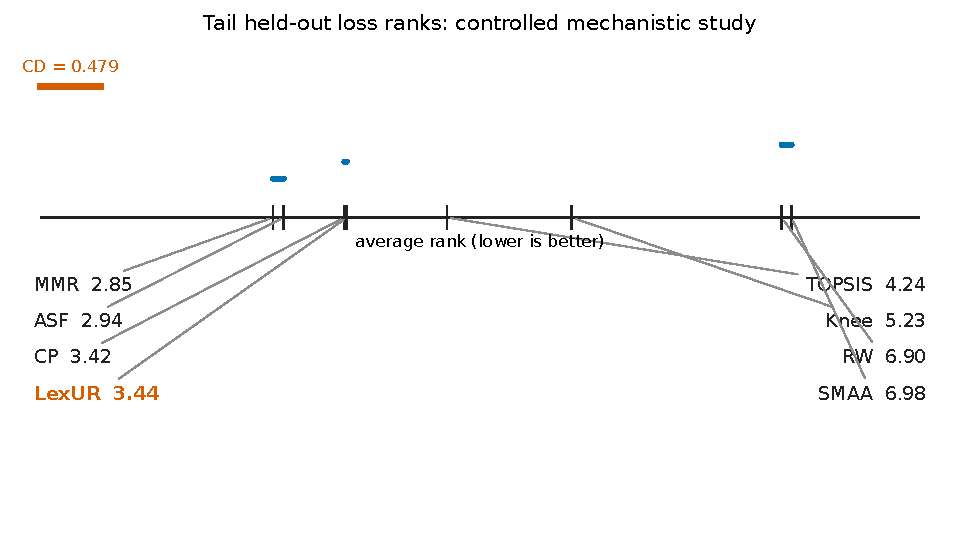
\includegraphics[width=0.85\textwidth]{cd_diagram.pdf}
\caption{Average ranks on tail (worst-case) held-out loss with Nemenyi critical
difference ($n=480$, $\alpha=0.05$, CD $=0.48$). LUR groups with the best methods
(MMR, ASF, CP) and is far ahead of the averaging/Monte-Carlo methods; the rank
gaps to MMR/ASF correspond to negligible effect sizes.}
\label{fig:cd}
\end{figure}

\subsection{Behaviour across preference families}
Table~\ref{tab:family} breaks the loss down by held-out family on a representative
setting (concave, $m=8$), including the two non-additive families. The structure
is a clear trade-off: averaging methods (TOPSIS, SMAA) are strong on linear
utilities but weak on the max-type families; ASF and MMR are the reverse---best on
Chebyshev/CES but worst on linear. LUR sits between the two camps: it removes much
of ASF's linear-utility weakness ($0.598$ vs $0.674$) while staying competitive on
the max-type \emph{and} the non-additive Choquet ($0.368$) and satisficing
($0.468$) families. We do \emph{not} claim LUR is the flattest profile---on this
setting CP is flatter and has the lowest overall mean ($0.404$)---only that LUR is
robust across additive and non-additive preferences without being tuned to any.

\begin{table}[t]
\centering\small
\caption{Held-out loss by preference family (concave, $m=8$, 30 replications),
including the non-additive Choquet and satisficing families. Lowest per column in
\textbf{bold}. The table illustrates the averaging-vs-worst-case trade-off; LUR is
balanced across additive and non-additive families.}
\label{tab:family}
\begin{tabular}{lccccccc}
\toprule
Method & linear & Cheby. & aug.\ ASF & CES & Choquet & satisfice & overall\\
\midrule
TOPSIS & \textbf{0.391} & 0.511 & 0.511 & 0.563 & 0.341 & 0.511 & 0.471\\
CP     & 0.486 & 0.458 & 0.458 & 0.440 & 0.307 & \textbf{0.278} & \textbf{0.404}\\
Knee   & 0.477 & 0.503 & 0.503 & 0.524 & 0.479 & 0.570 & 0.509\\
RW     & 0.403 & 0.519 & 0.519 & 0.569 & 0.379 & 0.552 & 0.490\\
ASF    & 0.674 & 0.434 & 0.434 & \textbf{0.329} & \textbf{0.288} & 0.388 & 0.425\\
SMAA   & 0.398 & 0.521 & 0.521 & 0.575 & 0.367 & 0.546 & 0.488\\
MMR    & 0.653 & 0.442 & 0.443 & 0.348 & 0.344 & 0.402 & 0.439\\
\textbf{LUR} & 0.598 & 0.454 & 0.454 & 0.374 & 0.368 & 0.468 & 0.453\\
\bottomrule
\end{tabular}
\end{table}

\subsection{Certificate regret and uniformity}
By construction LUR minimises the leximax of its certificate regret. Empirically
(concave, $m=8$) LUR attains worst-case certificate regret $0.708$, far below
every alternative (MMR $0.921$, CP $0.936$, ASF $0.953$, TOPSIS $0.974$), with one
of the most uniform regret profiles (sorted-disappointment std $0.219$, second to
MMR's $0.207$). This is by design---LUR optimises exactly this object---so it is a
consistency check, not an independent win; its decision value is that the
recommendation is \emph{auditable}.

\subsection{Robustness to redundant criteria}
We test the case motivating clustering: the DM's true preferences are over $c$
underlying criteria, each measured by several redundant (positively correlated)
objectives, with held-out utilities defined on the \emph{true} criteria. The
clustering recovers the redundancy groups essentially exactly.
Table~\ref{tab:redund} (four group structures $\times$ three geometries, 30
replications) shows LUR tied with ASF for best grouped loss and in the best group
on tail loss; the averaging and Monte-Carlo methods, which amplify redundant
groups, are $19$--$35\%$ worse on grouped loss (TOPSIS $0.332$, SMAA $0.413$ vs
LUR $0.268$). As discussed in \S\ref{sec:probes}, this reflects \emph{reduced},
not eliminated, redundancy sensitivity.

\begin{table}[t]
\centering\small
\caption{Redundant-objective benchmark (true preferences over the underlying
criteria; 4 group structures $\times$ 3 geometries, 30 replications). Grouped loss
measures de-redundification quality. Lower is better; best in \textbf{bold}.}
\label{tab:redund}
\begin{tabular}{lcc}
\toprule
Method & grouped loss & tail loss\\
\midrule
TOPSIS & 0.332 & 0.455\\
CP     & 0.317 & 0.423\\
Knee   & 0.322 & 0.489\\
RW     & 0.409 & 0.598\\
ASF    & \textbf{0.266} & 0.406\\
SMAA   & 0.413 & 0.603\\
MMR    & 0.295 & \textbf{0.387}\\
\textbf{LUR} & 0.268 & 0.391\\
\bottomrule
\end{tabular}
\end{table}

\subsection{Distinctness, dominated exclusion, ablation, sensitivity}
LUR and the SMAA recommender coincide on only $1.2\%$ of instances and select
alternatives a mean normalised distance $0.86$ apart: LUR is operationally a
different rule, not a re-description of acceptability analysis. Across 200
randomised trials with injected dominated points LUR never selected a dominated
alternative ($0/200$), confirming Corollary~\ref{cor:dom}. Ablation (concave,
$m=8$): dropping the singletons raises loss ($0.456\!\to\!0.483$) and worst-case
certificate regret ($0.701\!\to\!0.783$); a max-only family lowers mean loss to
$0.420$ but inflates certificate regret to $0.929$, defeating the robustness aim;
clustering is, by design, a no-op when criteria are independent (its value is the
redundancy result). LUR is insensitive to the clustering threshold $\theta$ over
$[0.3,0.9]$ across \emph{all four} geometries (Figure~\ref{fig:sens}, left). Under
nadir-estimation error the held-out loss of the chosen alternative stays stable
($\approx0.45$ up to $50\%$ error), though the \emph{identity} of the choice
changes increasingly often (Figure~\ref{fig:sens}, right), indicating near-ties
among good alternatives rather than quality loss.

\begin{figure}[t]
\centering
\begin{subfigure}{0.48\textwidth}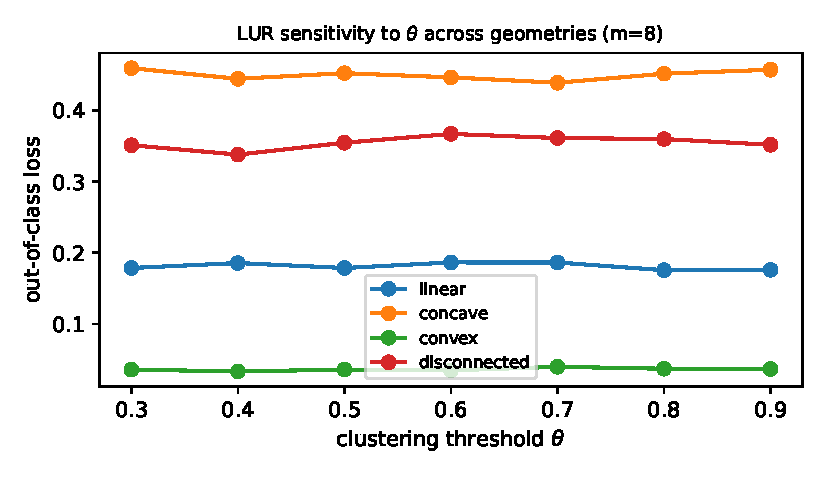
\includegraphics[width=\textwidth]{sensitivity_theta.pdf}\end{subfigure}
\hfill
\begin{subfigure}{0.48\textwidth}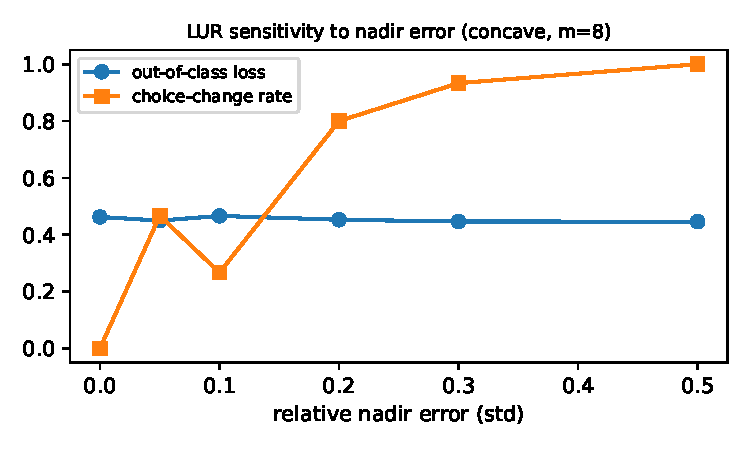
\includegraphics[width=\textwidth]{sensitivity_nadir.pdf}\end{subfigure}
\caption{Sensitivity of LUR. Left: held-out loss is flat in the clustering
threshold $\theta$ across all four geometries. Right: under nadir error the loss
stays stable while the recommendation changes more often (near-ties).}
\label{fig:sens}
\end{figure}

\subsection{Stochastic extension}
We validate the stochastic extension (Proposition~\ref{thm:stoch}) directly. On
noisy concave instances ($m=6$) we draw $n$ observations per criterion, form
plug-in means, and apply LUR; Figure~\ref{fig:stoch} reports how often the
resulting choice matches the noise-free LUR winner. Recovery rises monotonically
from $0.04$ at $n=1$ to $0.79$ at $n=100$, consistent with the consistency
statement (it does not reach $1$ because dense candidate sets contain near-ties,
exactly the situation the tolerance rule is designed for).

\begin{figure}[t]
\centering
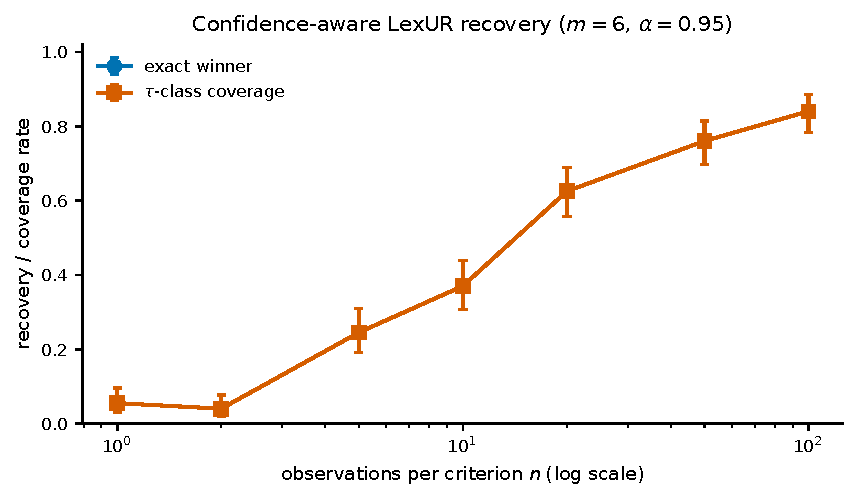
\includegraphics[width=0.6\textwidth]{stochastic_consistency.pdf}
\caption{Stochastic-LUR consistency: recovery rate of the noise-free winner vs.\
the number of observations per criterion (concave, $m=6$).}
\label{fig:stoch}
\end{figure}

\subsection{Pre-registered validation protocol and acceptance gates}
\label{sec:protocol}
To guard against confirmation bias we additionally ran a pre-registered protocol
(frozen config, single-command reproduction) on a deliberately broadened suite:
\textbf{eleven} methods (adding VIKOR, hypervolume contribution, and Chebyshev
minimax regret), \textbf{ten} held-out families spanning additive \emph{and}
non-additive preferences (adding sparse-linear, $L_p$, OWA, Choquet and
satisficing), Dirichlet weight shapes $\alpha\in\{0.2,1,5\}$, eight geometries and
$m$ up to $20$ ($2{,}400$ paired instances). The protocol fixes, in advance, a set
of \emph{acceptance gates}, each tied to one precise claim; we report the outcome
verbatim in Table~\ref{tab:gates} rather than only favourable numbers.

On this harder suite LUR has tail-loss rank $4.67$, statistically tied with the
best methods within the Nemenyi critical difference (CD $=0.31$): HV $4.27$,
ASF $4.65$, MMR $4.65$, LUR $4.67$, VIKOR $4.71$, ChebMMR $4.99$, then CP $5.32$,
TOPSIS $6.98$, knee $7.21$, RW $9.26$ and SMAA $9.30$ (Figure~\ref{fig:cdprot}).
A pre-registered \emph{non-inferiority} test (paired bootstrap, margin $0.01$
absolute \emph{or} $2\%$ relative) finds LUR non-inferior to both ASF and MMR
(upper 95\% CI bounds $0.004$ and $0.0025$), with negligible effect size
(Cliff's $\delta\le0.015$)---supporting ``practically equivalent to the best
robust scalarisations'' rather than ``better''. Direct computation is demonstrated
on a continuous linear MOP (LUR via sequential LPs uses $19$ solver calls and
\emph{no} front enumeration vs.\ $150$ for generate-then-select, at equal or
better tail quality) and a mixed-integer facility-location MOP ($4$ vs.\ $60$
solves for the same recommendation). The confidence-aware stochastic LUR attains
near-zero out-of-sample worst-criterion risk ($\approx0$) against $0.28$ for
TOPSIS and $0.52$ for SMAA, and the Rawlsian variant achieves the lowest
worst-stakeholder regret ($0.362$) and inequality (Gini $0.207$) among average-,
Nash- and max-min rules.

\begin{table}[t]
\centering\small
\caption{Pre-registered acceptance gates (reproduced at full scale). 9 PASS, 1 CHECK.}
\label{tab:gates}
\begin{tabular}{lll}
\toprule
Gate & Result & Evidence\\
\midrule
Dominated selections $=0$ & PASS & $0/150$ injections\\
Positive-affine invariance & PASS & $100\%$ identical\\
Nadir-error stability & CHECK & quality degr.\ $0.052$ (thr.\ $0.05$)\\
Non-inferior vs ASF (tail) & PASS & CI upper $0.004 < 2\%$ margin\\
Non-inferior vs MMR (tail) & PASS & CI upper $0.0025 < 0.01$ margin\\
Beats practical baselines (tail) & PASS & $\delta$: TOPSIS $.19$, CP $.06$, SMAA $.62$\\
Redundancy $<$ averaging (grouped) & PASS & $0.256$ vs $0.359$; cluster recovery $0.98$\\
Adaptive $\approx$ full (tail gap $\le0.01$) & PASS & gap $0.0096$\\
Direct computation (LP $+$ MILP) & PASS & $19$ vs $150$; $4$ vs $60$ solver calls\\
Stochastic LUR $\le$ deterministic (tail) & PASS & risk $\approx0$ vs $0.28/0.52$\\
\bottomrule
\end{tabular}
\end{table}

\begin{figure}[t]
\centering
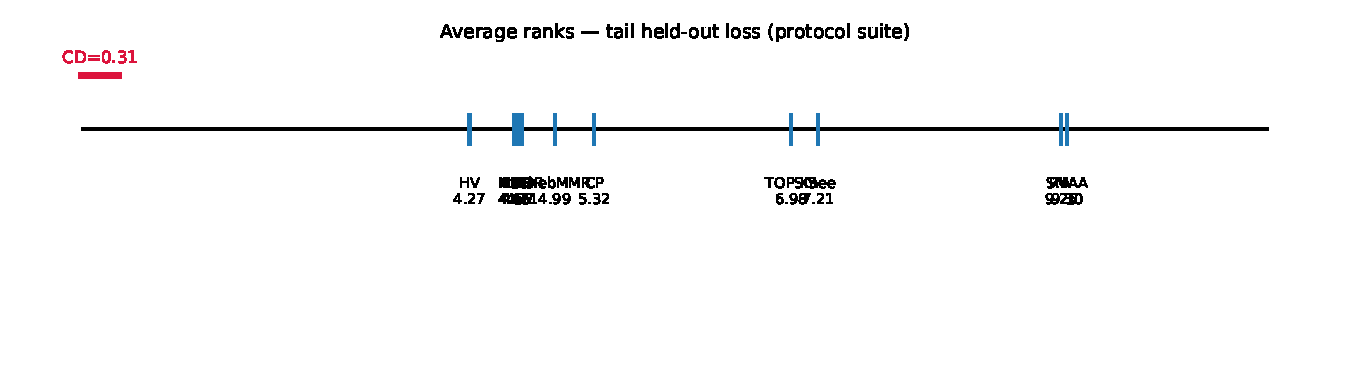
\includegraphics[width=0.92\textwidth]{cd_protocol.pdf}
\caption{Average ranks on tail held-out loss over the broadened protocol suite
(11 methods, 10 families, 8 geometries, $2{,}400$ instances; Nemenyi CD $=0.31$).
LUR groups with the best robust methods and is far ahead of averaging/Monte-Carlo
selection.}
\label{fig:cdprot}
\end{figure}

\subsection{Smart-grid dispatch case study}
We apply LUR to a six-objective stochastic 24-hour economic dispatch with ten
generators (cost, emissions, unreliability, ramping, non-renewable fraction, peak
gap) under Monte-Carlo renewable scenarios, yielding $163$ non-dominated dispatch
policies; the full dispatch model (demand profile, generator limits, ramping,
scenario generation) is specified in the released code.
Relative to the distance/averaging methods, LUR accepts a negligible increase in
\emph{mean} held-out loss ($0.103$ vs $0.100$) for a $23\%$ reduction in
\emph{worst-case} loss ($0.282$ vs $0.366$; knee $0.623$). Crucially it
\emph{explains} the choice: the certificate (Figure~\ref{fig:cert}) flags the
peak-shaving gap ($f_6$, regret $0.40$) and the non-renewable fraction ($f_5$,
$0.40$), then the ramping/peak coalition $\max(f_4,f_6)$ ($0.36$), telling the DM
not only which dispatch to adopt but where it remains fragile.

\begin{figure}[t]
\centering
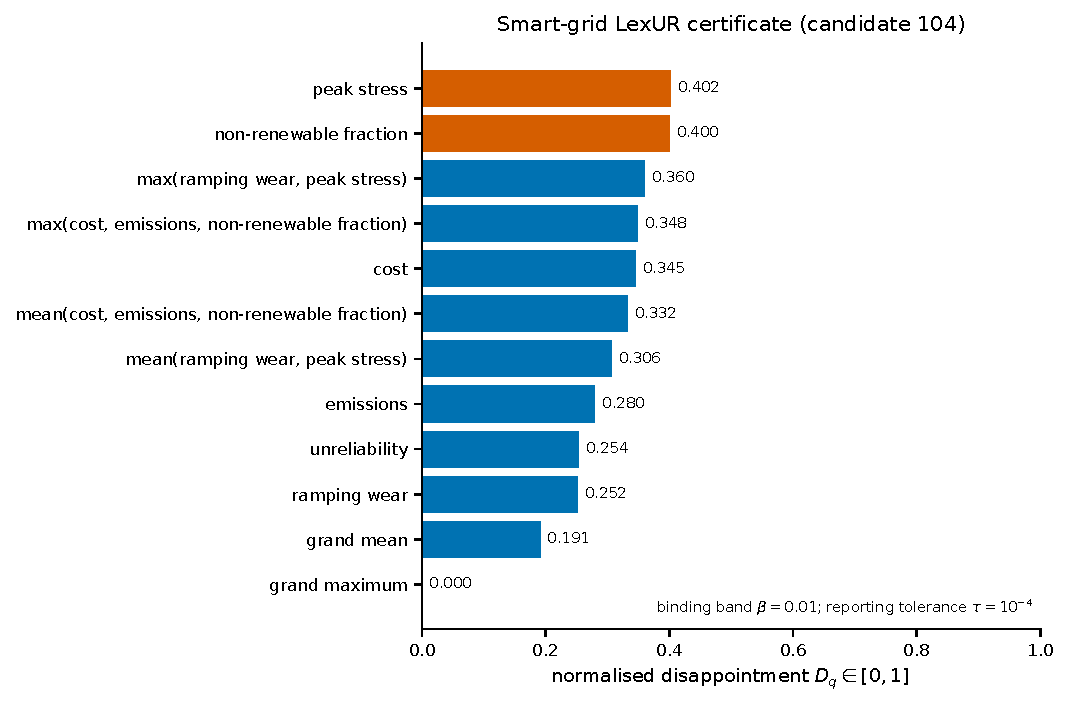
\includegraphics[width=0.7\textwidth]{certificate.pdf}
\caption{LUR regret certificate for the recommended smart-grid dispatch: the most
disappointed probes (peak gap $f_6$, non-renewable fraction $f_5$, and the
ramping/peak coalition) localise the fragility of the recommendation.}
\label{fig:cert}
\end{figure}

\section{Discussion and limitations}
\label{sec:disc}

\paragraph{What LexUR is, and is not.}
LexUR is a robust, certifiable decision rule. LexUR is competitive with the strongest robust scalarisations on tail held-out loss---non-inferior to achievement
scalarisation and sampled linear minimax regret (negligible effect sizes)---while on average-case loss the classical averaging
methods do better. LexUR's distinctive value is the \emph{combination} it offers
that no single competitor matches: worst-case robustness competitive with the
strongest robust scalarisations across additive \emph{and} non-additive
preferences (within one Nemenyi CD of MMR, VIKOR and ASF, though behind
the single-point hypervolume score on average rank), reduced sensitivity to redundant
criteria, an interpretable certificate, and natural stochastic and multi-stakeholder
extensions (the latter currently exploratory, \ref{app:rawlsian}). Where a DM cares only about average-case linear performance, a
weighted sum or SMAA is appropriate; where the DM cannot state preferences and
must defend a single robust, explainable choice, LexUR is designed for exactly that
situation. Table~\ref{tab:claims} provides a concise summary mapping the central claims of the paper to their theoretical or empirical evidence.

\begin{table}[h]
\centering\small
\caption{Claim-evidence matrix mapping theoretical properties and empirical findings to their supporting evidence.}
\label{tab:claims}
\begin{tabular}{p{5cm}p{7cm}}
\toprule
Claim & Evidence \\
\midrule
Pareto compatibility & Theorem~\ref{thm:pareto} (general) and Theorem~\ref{thm:nonneg} (non-negative probes) \\
Existence and completeness & Theorem~\ref{thm:exist} \\
Tolerance-rule stability & Theorem~\ref{thm:stab} (margin condition) \\
Reduced redundancy bias & Table~\ref{tab:redund} (grouped loss) \\
Robustness on tail held-out loss & Figure~\ref{fig:cd} and Table~\ref{tab:main} \\
Stochastic consistency & Proposition~\ref{thm:stoch2} and Figure~\ref{fig:stoch} \\
Smart-grid applicability & \ref{app:smartgrid} and Figure~\ref{fig:cert} \\
\bottomrule
\end{tabular}
\end{table}

\paragraph{Relationship to existing rules.}
LexUR generalises rather than replaces. A single grand-maximum probe recovers the
Chebyshev/ASF rule; a single weighted-mean probe recovers a weighted sum, and the
grand mean recovers its equal-weight case; the
singleton family recovers lexicographic maximin of normalised regret. The
empirical question is whether the richer adaptive family helps, and the answer is
that it does on redundant and asymmetric problems while not materially hurting on
the tested standard geometries.

\paragraph{Independence of Irrelevant Alternatives (IIA) and Set-Dependence.}
Because both the normalisation bounds ($\ideal, \nadir$) and the probe anchors ($q^\star, q^w$) are computed empirically over the active candidate set $A$, LexUR does not satisfy Independence of Irrelevant Alternatives (IIA). Adding or removing a non-selected, non-dominated alternative that defines an extremum shifts the normalisation for \emph{all} alternatives, which can change the sorted disappointment vectors and cause rank reversal. This is structurally the same vulnerability identified in TOPSIS (\S\ref{sec:intro}). This set-dependence explains the high winner-flip rates observed in our nadir-sensitivity experiments (Table~\ref{tab:gates}). We must therefore unequivocally state: unless normalisation bounds are fixed \emph{a priori} by the decision maker, point-estimate normalisation should be avoided in favour of the interval/stability analysis (Option B) defined in \S\ref{sec:core}. Deploying LexUR with conservative interval bounds is mandatory when stability against candidate-set perturbations is required.

\paragraph{The Certificate's Decision Value.}
While robust scalarisations like ASF provide similar worst-case guarantees, LexUR's distinct value lies in its auditable certificate. A standard sensitivity sweep over ASF reference points or a SMAA acceptability index reveals \emph{how often} an alternative wins, but does not explain \emph{why} it loses in specific contexts. In contrast, the LexUR certificate explicitly isolates the binding constraints: it names the specific declared probe (e.g., ``the average of cost and emissions'') that forces the maximum disappointment, giving the decision maker a direct semantic justification for the compromise that opaque distributional indices omit. Figure~\ref{fig:certconcept} shows the anatomy of such a certificate.

% Conceptual anatomy of a regret certificate
\begin{figure}[t]
\centering
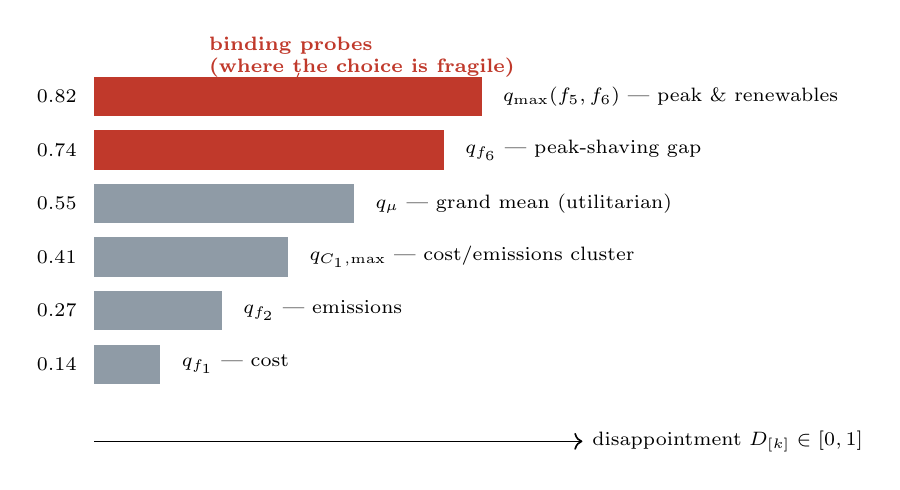
\begin{tikzpicture}[x=1cm,y=1cm]
\def\bh{0.5} % bar height
% horizontal bars, sorted descending, top = most binding
\foreach \i/\v/\lab/\hot in {%
   0/0.82/{$q_{\max}(f_5,f_6)$ — peak \& renewables}/1,
   1/0.74/{$q_{f_6}$ — peak-shaving gap}/1,
   2/0.55/{$q_{\mu}$ — grand mean (utilitarian)}/0,
   3/0.41/{$q_{C_1,\max}$ — cost/emissions cluster}/0,
   4/0.27/{$q_{f_2}$ — emissions}/0,
   5/0.14/{$q_{f_1}$ — cost}/0}{
   \pgfmathsetmacro\yy{-\i*(\bh+0.18)}
   \ifnum\hot=1
     \fill[lurcrimson] (0,\yy) rectangle ++(\v*6,\bh);
   \else
     \fill[lurslate!55] (0,\yy) rectangle ++(\v*6,\bh);
   \fi
   \node[anchor=west, font=\scriptsize] at (\v*6+0.15,\yy+\bh/2) {\lab};
   \node[anchor=east, font=\scriptsize] at (-0.1,\yy+\bh/2) {\pgfmathprintnumber{\v}};
}
% axis
\draw[->,line width=0.6pt] (0,-6*0.68-0.05) -- (6.2,-6*0.68-0.05)
   node[right,font=\scriptsize]{disappointment $\reg_{[k]}\in[0,1]$};
% brace-like annotation for binding probes
\node[lurcrimson, font=\scriptsize\bfseries, align=left] at (3.4,0.75)
   {binding probes\\\scriptsize(where the choice is fragile)};
\draw[lurcrimson,-{Stealth[length=1.8mm]}] (2.6,0.55) -- (2.4,0.05);
\end{tikzpicture}
\caption{Anatomy of a regret certificate. The recommendation is reported with its
probe disappointments sorted worst-first; the top, highlighted entries are the
\emph{binding probes} that drive the worst-case regret and localise the fragility
of the choice (illustrative labels follow the smart-grid case of \S\ref{sec:exp}).}
\label{fig:certconcept}
\end{figure}


\paragraph{Scope, Parameters, and Limitations.}
LexUR is a lexicographic minimax regret selector. It complements exploratory tools like SMAA by providing a single, auditable point recommendation when the DM must defend a robust choice. The framework relies on several explicit choices, summarised in Table~\ref{tab:params}. LexUR's contribution is that these choices are declared and separated from the final recommendation.

\begin{table}[h]
\centering\small
\caption{Consolidated list of LexUR parameters, their roles, and recommended defaults.}
\label{tab:params}
\begin{tabular}{lllp{6cm}}
\toprule
Param & Role & Default & Note \\
\midrule
$\ideal, \nadir$ & Normalisation bounds & Empirical over $A$ & Must use fixed \emph{a priori} bounds if IIA/stability is required. \\
$\Q$ & Probe family & Adaptive family & Defines the semantic interpretations of preference. \\
$\theta$ & Clustering threshold & $0.6$ & Empirically insensitive over $[0.4, 0.8]$. \\
$\tau$ & Leximax tolerance & $10^{-4}$ & Set to the scale of the disappointment estimation error. \\
$\varepsilon_q$ & Degeneracy / range floor & $10^{-6}$ & Minimum admissible probe/criterion active range; below it the probe/criterion is flagged degenerate. The empirical stability margin $\Delta$ of Theorem~\ref{thm:stab} is an instance property, not a tunable parameter. \\
$\alpha$ & Stochastic confidence & $0.95$ & Used only in the stochastic extension (\S\ref{sec:ext}). \\
\bottomrule
\end{tabular}
\end{table}

\paragraph{Threats to validity.}
The held-out families, though disjoint from the probes, are themselves a modelling
choice; we mitigate this by spanning linear, Chebyshev, ASF and CES forms and by
reporting per-family results. Candidate sets are synthetic but cover eight
audit geometries, with four canonical geometries used in the mechanistic study,
and the dispatch illustration is also synthetic; extending to a wider
library of real MCDA datasets is future work.

\paragraph{Interactive elicitation using certificates.}
The certificate could support a future interactive workflow in which the DM
reviews the binding probes and revises the declared family. For example, a DM
might relax a cost-focused probe after seeing its effect on the recommendation,
after which LexUR can be recomputed. This possibility has not been evaluated here:
removing a separating singleton can weaken Pareto-exclusion guarantees, so an
interactive protocol would require explicit safeguards and user validation.

\paragraph{Future work.}
Natural next steps include large-scale empirical validation of the continuous direct formulations (\S\ref{sec:direct}) on high-dimensional problems; and full development and evaluation of the exploratory Rawlsian multi-stakeholder variant. Finally, extending the family to include non-linear probes would significantly broaden LexUR's expressive power. For instance, capturing Cobb-Douglas structures (constant elasticity of substitution) could be achieved by evaluating linear probes in log-transformed criterion space, while modelling threshold-based satisficing preferences with interaction terms would require explicitly incorporating boolean conditionals into the anchor computations.

\section{Conclusion}
\label{sec:conc}

We have presented the Leximax Universal-Regret core, a Pareto-compatible decision
rule that replaces the efficient set as the final object of multicriteria analysis
with an auditable certificate. LexUR operates as a lexicographic minimax regret selection rule: it ranks alternatives by the
lexicographically sorted vector of normalised achievement shortfalls over a declared family of
monotone probes, and returns a robust stability class (often a singleton recommendation) together with an
explanation of where it remains fragile. We proved existence and completeness,
Pareto compatibility \emph{under a separation condition}, dominated-solution
exclusion, stability of the tolerance-based rule under bounded perturbations, and
a disappointment-perturbation bound with explicit constants, and we gave a
redundancy-aware, correlation-clustering probe construction that keeps the family
linear in the number of criteria. A replicated held-out study over ten preference
families and a stochastic smart-grid case showed that LexUR attains
worst-case robustness competitive with the strongest robust
scalarisations---performing non-inferiorly to achievement scalarisation and
sampled minimax regret, while a single-point hypervolume score ($\mathrm{HV}_1$) obtains the best average rank---and does
so while reducing sensitivity to redundant criteria, certifying
its choices, and extending naturally to noisy criteria.

The central message is that robust, explainable selection can be obtained from a declared family of monotone questions rather than from elicited scalarisation weights. In structured cases (e.g.\ linear MOPs) LexUR can sometimes be computed directly, without front enumeration; in the general case, however, it remains primarily a \emph{post hoc} candidate-set selector, and we make no claim that it replaces front generation universally. This robustness also relies entirely on the reliability of the supplied normalisation bounds; if true nadirs are uncertain, the framework must be deployed conservatively using interval estimates. By relocating preference choices into a declared class of questions, LexUR turns a candidate set into a defensible,
explainable recommendation---a low-disappointment compromise across the declared
interpretations of the criteria, accompanied by a certificate that reports which
questions remain most binding.

\paragraph{Reproducibility.}
All code, generated data, and scripts that regenerate every table and figure in
this paper are released in an open-source repository (URL withheld to preserve
anonymity during review; it will be provided in the camera-ready version),
including the four-geometry benchmark, the redundancy
benchmark, the statistical tests, the sensitivity analyses, and the smart-grid
case study.


\bibliographystyle{plainnat}
\bibliography{refs}

\appendix
\section{Smart-grid economic dispatch formulation}
\label{app:smartgrid}
The case study in \S\ref{sec:exp} evaluates a 24-hour multi-objective economic dispatch on a synthetic 14-generator instance constructed using the IEEE 14-bus demand/generator template. To prevent any misreading of the model's fidelity, we describe the actual implementation precisely. it is deliberately a lightweight \emph{priority-dispatch heuristic}, \emph{not} a binary unit-commitment MILP and \emph{not} a network-constrained AC/DC optimal power flow. It is an \emph{aggregate} (single-bus) dispatch: the IEEE 14-bus data supplies the demand profile and the generator cost/emission/ramp template only, and no nodal power-flow, transmission-limit, line-loss, or binary commitment constraints are modelled (the dispatch balances the hourly demand $d_t(\omega)$ directly).

\paragraph{Candidate policy and dispatch rule.}
A candidate policy is a non-negative \emph{dispatch-priority} vector $\pi\in\mathbb{R}^{14}_{\ge 0}$, normalised to $\sum_g\pi_g=1$. there are no binary commitment variables, and all generators are treated as available (renewable units have hour- and scenario-dependent available capacity). For each hour $t$ and scenario $\omega$, let $C_{gt}(\omega)$ be the available capacity ($C_{gt}=P_g^{\max}$ for thermal units, and the renewable cap scaled by the realised solar/wind availability for renewable units). The dispatch is computed by a two-pass priority rule:
\begin{equation}
p_{gt}(\omega)=\min\!\bigl(\pi_g\,d_t(\omega),\,C_{gt}(\omega)\bigr)\ \text{(nominal share, capped)},
\end{equation}
after which any residual demand $d_t(\omega)-\sum_g p_{gt}(\omega)$ is filled greedily in proportion to the remaining headroom $C_{gt}(\omega)-p_{gt}(\omega)$, up to capacity. No ramp constraint is enforced. inter-hour ramping is \emph{measured} as the wear objective below, not constrained. Renewable energy beyond what is dispatched is simply not used (there is no explicit curtailment variable). Any demand that still cannot be met is recorded as load shedding,
\begin{equation}
s_t^{\mathrm{shed}}(\omega)=\max\!\Bigl(d_t(\omega)-\textstyle\sum_g p_{gt}(\omega),\,0\Bigr),
\end{equation}
which feeds the unreliability objective. Every sampled policy is therefore \emph{feasible by construction}: capacity violations are impossible (dispatch is capped) and any supply shortfall is absorbed as load shedding rather than discarded or repaired.

The six objectives to be minimised are given below, each up to a fixed positive
scaling constant that does not affect ranking or active-set normalisation. Let
$G_{\mathrm{th}}$ and $G_{\mathrm{ren}}$ denote the thermal and renewable generator
sets, $c_g,e_g$ the fuel-cost and emission coefficients, and $R_g$ the ramp scale.
\begin{enumerate}
    \item \textbf{Cost:} $f_1(x)=\mathbb{E}_\omega\!\left[\sum_{t}\sum_{g} c_g\,p_{gt}(\omega)\right]$.
    \item \textbf{Emissions:} $f_2(x)=\mathbb{E}_\omega\!\left[\sum_{t}\sum_{g} e_g\,p_{gt}(\omega)\right]$.
    \item \textbf{Unreliability:} Loss-of-load probability, the fraction of scenarios in which any load is shed,
    \[ f_3(x)=\frac{1}{|\Omega|}\sum_{\omega\in\Omega}\mathbf 1\!\left[\sum_t s_t^{\mathrm{shed}}(\omega)>0\right]. \]
    \item \textbf{Ramping wear:} expected ramp magnitude normalised by the per-generator ramp scale $R_g$ (a wear normaliser, \emph{not} an enforced ramp limit),
    \[ f_4(x)=\mathbb{E}_\omega\!\left[\sum_{g}\sum_{t>1} \frac{|p_{g,t}(\omega)-p_{g,t-1}(\omega)|}{R_g}\right]. \]
    \item \textbf{Non-renewable fraction:} expectation \emph{of the per-scenario ratio} of thermal to total dispatched energy (an expectation of a ratio, not a ratio of expectations),
    \[ f_5(x)=\mathbb{E}_\omega\!\left[\frac{\sum_{t}\sum_{g\in G_{\mathrm{th}}} p_{gt}(\omega)}{\sum_{t}\sum_{g} p_{gt}(\omega)+\varepsilon}\right]. \]
    \item \textbf{Peak stress:} a peak-shaving proxy equal to the peak demand scaled by the priority weight \emph{not} pre-allocated to thermal generators,
    \[ f_6(x)=d^{\mathrm{peak}}\,\max\!\Bigl(1-\textstyle\sum_{g\in G_{\mathrm{th}}}\pi_g,\,0\Bigr). \]
\end{enumerate}

Each candidate policy is evaluated by Monte-Carlo sample-average approximation over $20$ renewable scenarios drawn from the scenario model. The candidate set is generated \emph{a priori}, independently of LexUR: we sample a population of $250$ dispatch policies as Dirichlet-weighted generator allocations ($\mathrm{Dir}(0.6\cdot\mathbf 1)$ over the $14$ generators, seed $2024$), evaluate each under the scenarios, and retain the $163$ non-dominated policies as the efficient candidate set. No evolutionary operators (selection, crossover, mutation) are used. a population metaheuristic such as NSGA-II could be substituted without changing LexUR's role as a post-hoc selector. All parameter values (generator data, costs, emissions, ramp-wear coefficients $R_g$, and scenario bounds), random seeds, and the exact scenario count are fixed in the open-source repository. This formulation serves as an illustrative application of the robust certificate framework.

\section{Multi-stakeholder (Rawlsian) exploratory variant}
\label{app:rawlsian}

Let $\mathcal U=\{1,\dots,U\}$ index stakeholders, each with importance weights
$w_u\in\Delta^m$ inducing a stakeholder-specific disappointment $\reg_q^u(x)$.
An exploratory \emph{Rawlsian LUR} applies the leximax order to the worst-stakeholder
disappointments, $\max_{u}\reg_{q}^u(x)$.
It maintains natural fairness properties such as anonymity and worst-stakeholder protection. A full treatment of this extension is beyond the scope of this paper, but we include this preliminary formulation to demonstrate the flexibility of the regret-certificate framework.


\end{document}
